\chapter{System Implementation} \label{chapter:implementation}

This chapter presents the UAchado intelligent \ac{lfms} implementation, covering technical solutions, code details, architectural patterns, and production-ready deployment infrastructure. Following the architectural evolution from Chapter \ref{chapter:methodology}, the implementation uses a modular monolith that maintains microservices principles while reducing operational complexity. The chapter focuses on architectural decisions, code structure, and integration patterns, concluding with containerized architecture, monitoring infrastructure, and operational procedures.

% ____________________ Database Implementation and Data Models ____________________ %

\section{Database Implementation and Data Models} \label{section:database_implementation}

The database uses PocketBase, an open-source Backend-as-a-Service platform that provides SQLite\footnote{\url{https://sqlite.org/}}-based storage with authentication, real-time synchronisation, and file handling. The 17-collection schema evolved iteratively to support multi-tenant \ac{lfms} requirements with \ac{ai}-powered matching.

Database architecture follows a community-centric, multi-tenant approach for data isolation with controlled cross-community processes. It extends PocketBase's authentication with \ac{rbac}, supporting three user types: ordinary users, local managers, and system administrators. Community-based scoping restricts access to authorised items and communications, while indexing and queue processing handle \ac{ai} tasks efficiently. Permissions control access at the collection and record levels.

The 17-collection schema is organised into five functional categories. User management employs four collections for hierarchical role-based authentication, while community management uses four collections for organisational boundaries and physical locations. Core functionality relies on five collections managing the complete item lifecycle and \ac{ai} matching. Communication encompasses three collections for community and direct messaging, and system tasks use two collections for notifications and audit trails. Each category serves specific functional requirements while maintaining data isolation through community-based scoping.

\subsubsection{Relationship Design and Data Integrity}

Database implementation uses a hierarchical relationship model with user inheritance through role-specific collections referencing the base \texttt{users} collection. The community hierarchy enables data scoping where communities own managing points that store items. Item lifecycle tracking uses dynamic foreign keys to record initial storage and transfers between points.

Indexing uses unique constraints to prevent inconsistencies and composite indexes for multi-table queries. Queue processing employs specialised indexes including \texttt{(community\_id, status)} for community-based processing and \texttt{(priority DESC, queued\_at ASC)} for priority-based fairness. Relationship indexes optimise frequently accessed join operations between collections.

The complete entity relationship diagram illustrating the 17-collection schema with all foreign key relationships is provided in Appendix \ref{app:database_schema}.

\subsubsection{File Storage and Media Management}

File storage uses PocketBase's built-in features for image uploads with media type restrictions and 10MB size limits. File access integrates with permissions, restricting users to images from their authorised communities.

\subsection{Data Access Layer} \label{subsection:data_access_layer}

The data access layer uses a repository pattern to abstract business logic from PocketBase operations. Repository classes manage database interactions, \ac{http} clients, and data transformations following the \ac{rsr} pattern. Each domain entity has a dedicated repository class that encapsulates data access functions. Key repositories include \texttt{FoundItemRepository} and \texttt{ReportedItemRepository} for item \ac{crud} tasks, \texttt{AuthRepository} for multi-collection user authentication, \texttt{ItemMatchRepository} for \ac{ai}-powered matching processes, and \texttt{ItemProcessingQueueRepository} for asynchronous processing with priority-based queuing. Community-related repositories (\texttt{CommunityRepository}, \texttt{LMPRepository}, \texttt{OUCRepository}) handle organizational data, providing a consistent interface for all database operations.

The \ac{http} client configuration uses \texttt{httpx}\footnote{\url{https://www.python-httpx.org/}} for asynchronous PocketBase communication with connection pooling, 30-second timeouts, and Bearer token authentication\footnote{\url{https://www.ietf.org/rfc/rfc6750.txt}}. Error handling transforms network issues into appropriate \ac{http} status codes: 408\footnote{\url{https://httpstatuses.com/408}} for timeouts and 503\footnote{\url{https://httpstatuses.com/503}} for connection errors, preserving original responses for proper error propagation.

Query optimisation improves performance through several techniques tailored to PocketBase's features. The implementation uses consistent pagination with 30 items per page by default, parameterised filtering for multi-tenant isolation and workflow management, and strategic relationship expansion using the \texttt{expand} parameter to reduce round-trip requests. Sorting functions support \ac{ui} requirements like creation time ordering and \ac{ai} result display through confidence scores. Table \ref{tab:query_optimization} provides a comparison of the implemented optimization techniques, their specific use cases, and measured performance impacts.

\begin{table}[htbp]
    \centering
    \caption[Query Optimization Techniques]{Query Optimization Techniques: Implementation, Use Cases, and Performance Impact}
    \label{tab:query_optimization}
    \footnotesize
    \begin{tabular}{p{2.2cm}p{4.5cm}p{6cm}}
        \hline
        \textbf{Technique} & \textbf{Implementation} & \textbf{Use Cases} \\
        \hline
        Pagination & PocketBase \ac{api} with \texttt{page}, \texttt{perPage} parameters (default 30) & Found items retrieval, reported items listing, community management \\
        \hline
        Filtering & URL-encoded filter strings with PocketBase syntax & Community-based filtering, status filtering, category selection \\
        \hline
        Relationship Expansion & \texttt{expand} parameter for related data fetching & Match queries with item details, user-community relationships \\
        \hline
        Sorting & PocketBase \texttt{sort} parameter with database-level ordering & Queue processing priority, match confidence scores, creation timestamps \\
        \hline
        Connection Reuse & HTTP client with persistent connections & Repository layer requests, authentication calls, file operations \\
        \hline
        Error Handling & Timeout management and retry mechanisms & Network timeouts (408), connection errors (503), service degradation \\
        \hline
    \end{tabular}
\end{table}

Data access addresses several architectural challenges inherent to working with PocketBase's SQLite backend. Without distributed transactions, the system employs compensating actions and state management for multi-step operations. The item matching process exemplifies this approach by deleting pending matches before requeuing updated items, while queue operations use atomic state transitions where possible, supplemented by retry mechanisms for transient failures. Error recovery preserves successful operations while logging and potentially retrying failures, maintaining system continuity despite individual operation problems.

PocketBase's \ac{rest} \ac{api} supports an architecture for future real-time features via WebSockets\footnote{\url{https://en.wikipedia.org/wiki/WebSocket}}. The repository structure accommodates selective updates based on permissions and community membership, with the current implementation focusing on reliable \ac{http} communication, providing a pathway for real-time enhancement when operational requirements justify additional features.

Authentication token management reduces redundant PocketBase calls through automatic token refresh with 30-second buffers and in-memory caching. It improves performance during active sessions while maintaining security through proper lifecycle management. The architecture also supports future caching strategies for frequently accessed data with time-based expiration and invalidation patterns.

Error handling categorises failures into transient and permanent types, each with appropriate recovery strategies. Network timeouts and temporary unavailability trigger retry mechanisms that avoid overwhelming PocketBase during degradation periods. In contrast, authentication failures and validation errors propagate immediately with detailed context, enabling proper error responses to clients.

Data integrity mechanisms operate at multiple levels throughout the access layer. Input validation checks that data conforms to expected formats before database operations, and foreign key verification maintains referential integrity across collections. The layer handles data transformation between application objects and PocketBase formats automatically, with schema evolution support allowing for controlled database transitions. Version checking and migration capabilities also abstract PocketBase complexities from the application layer, providing smooth updates as the system evolves.

% ____________________ Core Services Implementation ____________________ %

\section{Core Services Implementation} \label{section:core_services}

Core services expose functionality through FastAPI with 11 specialised routers handling authentication, item management, community operations, matching workflows, and administrative functions. Figure \ref{fig:fastapi_routers} illustrates the router architecture, showing how each router specialises in specific domain responsibilities.

\begin{figure}[htbp]
    \centering
    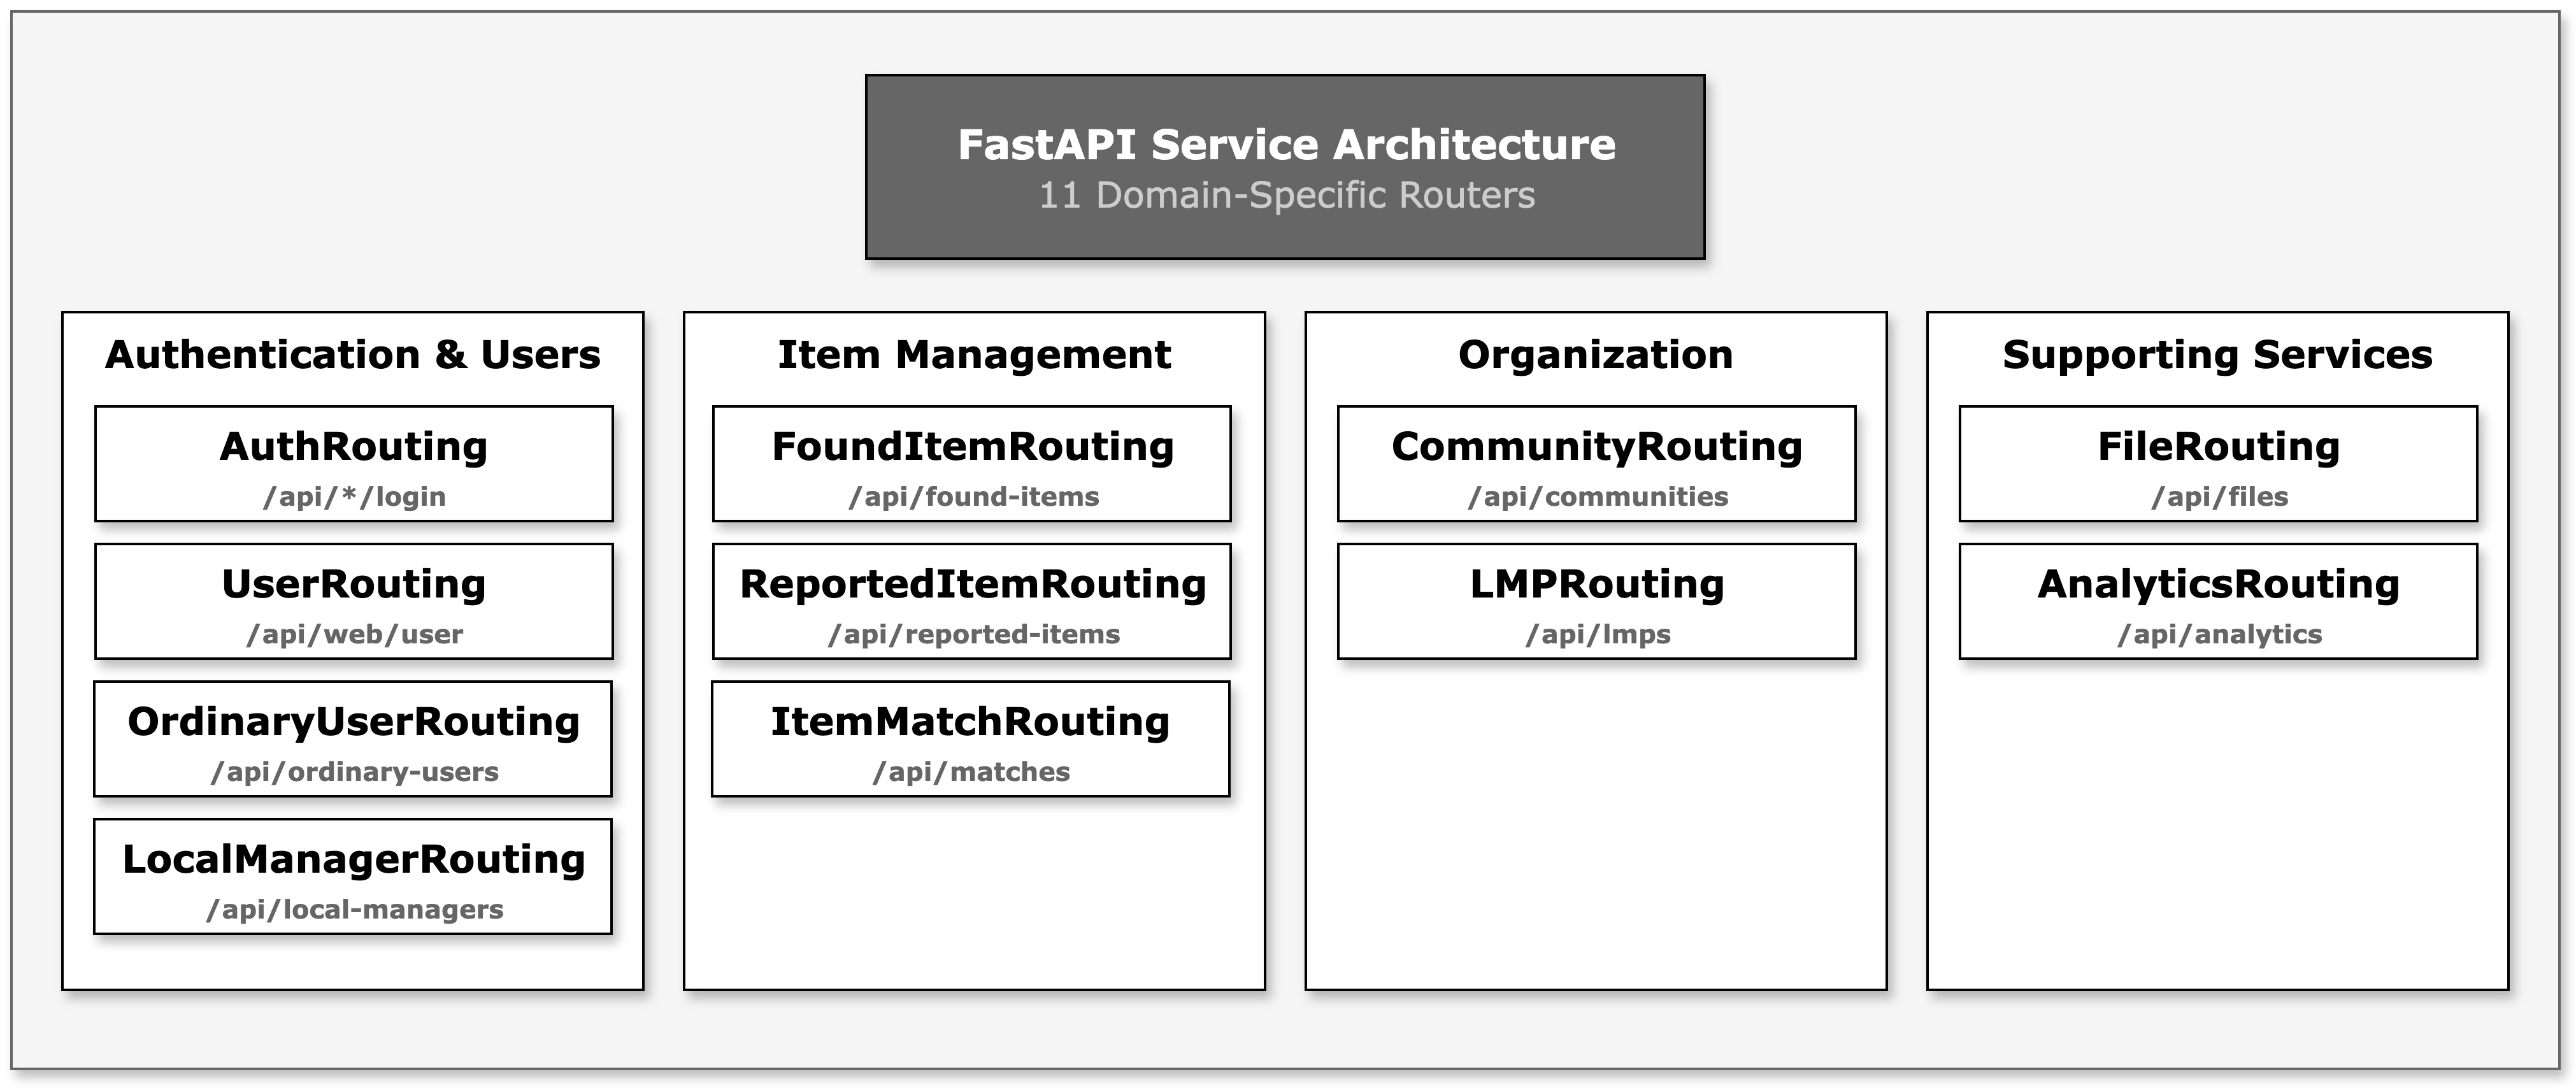
\includegraphics[width=\textwidth]{figs/chapter4/fastapi_routers.png}
    \caption[FastAPI Routers Architecture]{FastAPI routers architecture showing the 11 domain-specific routers organized into four functional groups: Authentication \& User Management (4 routers), Item Management (3 routers), Organization (2 routers), and Supporting Services (2 routers)}
    \label{fig:fastapi_routers}
\end{figure}

\subsection{Authentication Service Code} \label{subsection:auth_service}

Authentication distinguishes three user types: ordinary users who access the mobile application, local managers who operate the web dashboard, and administrators who have full privileges. Each role maps to a distinct PocketBase collection with specific authentication endpoints. Ordinary users access \texttt{/api/mobile} with public self-registration, while managers and administrators use \texttt{/api/web} with controlled access.

Authentication validates \acp{jwt} through Base64 \acs{url}-safe decoding and handles automatic refresh with 5-minute expiration thresholds, while in-memory caching provides time-to-live management for improved performance.

Token validation applies a 30-second expiration buffer to determine when tokens should be considered expired, with graceful fallback when refresh attempts fail but tokens remain valid. The implementation incorporates cleanup mechanisms to prevent memory leaks. Token caching reduces authentication requests to PocketBase during active user sessions.

FastAPI dependencies provide declarative security across \ac{api} endpoints. The user authentication dependency extracts and validates Bearer tokens from request headers, checking the token cache before decoding \ac{jwt} payloads. Role-specific dependencies support both single-role requirements and multiple acceptable roles for flexible access control. Convenience functions handle common administrative patterns and manager-level access requirements. The dependency system creates user authentication objects containing user identifiers, email addresses, collection names, and community associations where applicable. Figure \ref{fig:jwt_auth_sequence} illustrates the complete JWT authentication flow, including token validation, caching mechanisms, and the refresh logic.

\begin{figure}[htbp]
    \centering
    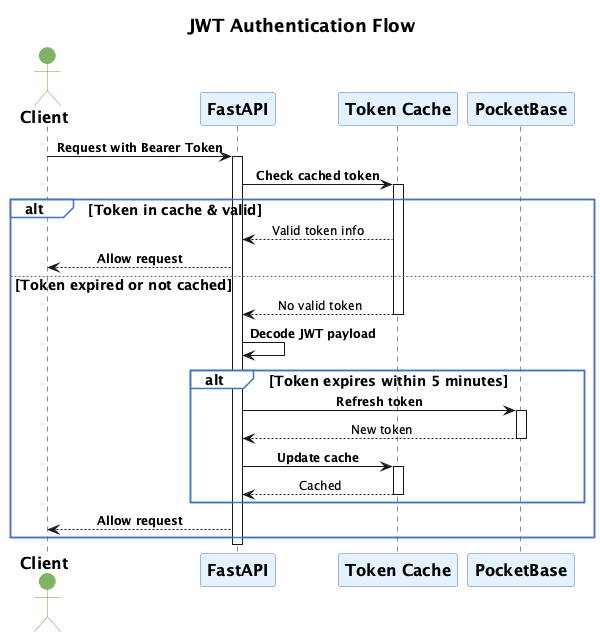
\includegraphics[width=0.8\textwidth]{figs/chapter4/jwt_auth_simple.png}
    \caption[JWT Authentication Flow]{JWT authentication flow showing token validation, caching, and refresh logic with PocketBase integration}
    \label{fig:jwt_auth_sequence}
\end{figure}

\subsection{Item Management Service} \label{subsection:item_management_service}

Item management orchestrates the complete lifecycle of lost and found items through parallel implementations that handle both found and reported items with identical patterns. The service incorporates intelligent processing, automated security classification, and asynchronous event handling while maintaining strict community-based access control.

Lifecycle management includes retrieval, creation, modification, and deletion operations. When users submit new items, validation occurs against predefined category enumerations, security levels are automatically determined based on item characteristics, and asynchronous \ac{ai} processing begins without blocking the main request flow.

Update mechanisms implement intelligent re-processing logic that evaluates whether modifications to item properties warrant renewed \ac{ai} analysis. When users modify descriptions or categories - properties that fundamentally affect the matching algorithm - the system automatically requeues items for processing. Query construction supports suitable filtering, including fuzzy text matching for flexible search functionality, boolean state filtering for retrieval status tracking, and location filtering that considers both delivery points and current storage locations.

\subsubsection{Image Processing and \ac{ai} Integration}

Image processing uses multimodal \ac{ai} through the \ac{llava} model for automated content analysis and classification. When users upload images, detailed object descriptions are generated by analysing visual content and categories are automatically assigned through pattern matching against the classification taxonomy. To improve performance when handling multiple images simultaneously, the system implements a batch processing strategy that reduces overhead and improves throughput.

\subsubsection{Security Classification and Access Control}

Security frameworks implement an automated three-tier classification system that analyses item properties to determine appropriate visibility levels. High-security items, including electronics, valuable objects, and other personal documents, receive maximum protection with masked images and obscured descriptions for standard users. Medium-security items, such as bags and sports equipment, maintain image visibility while restricting location details to prevent unauthorised retrieval attempts. Low-security items, including clothing and books, operate with complete transparency, balancing accessibility with reasonable privacy protection.

Access control operates through community-based scoping enforced at the data access layer, so all database operations automatically filter results based on user community membership. \ac{rbac} determines which data fields and operations each user type can access, creating a flexible yet secure authorisation framework.

\subsubsection{Event-Driven Queue Integration}

Queue management implements a facade pattern that coordinates multiple specialised services handling continuous background processing, batch operations for efficiency, and monitoring.

When \ac{ai} services become unavailable, the implementation gracefully degrades to basic functionality while queuing items for later processing. Detailed logging captures operational information for debugging and performance analysis, while structured exception handling maintains clean error propagation through service components, managing high-throughput processing workloads while preserving data consistency and stability.

\subsection{Request Routing and Proxy Configuration} \label{subsection:reverse_proxy_gateway}

The implementation uses a reverse proxy pattern with Nginx rather than a traditional \ac{api} gateway. This design choice favours simplicity over traditional gateway functionality, creating a single entry point for all services.

The Nginx-based reverse proxy uses path-based routing with static upstream configuration. Request routing follows a clear pattern: \texttt{/api/*} routes to the FastAPI backend on port 8000, \texttt{/pb/*} directs to PocketBase administration on port 8090, and \texttt{/monitoring/*} connects to Grafana dashboards on port 3000. Figure \ref{fig:network_topology} illustrates the complete network topology and routing architecture.

Configuration creates upstream connections with keepalive pools configured for each service type. FastAPI receives 32 keepalive connections for high-throughput \ac{api} operations, while PocketBase administration uses 16 connections for moderate administrative traffic. Connection reuse reduces TCP overhead and improves response times during sustained operation.

\begin{figure}[htbp]
    \centering
    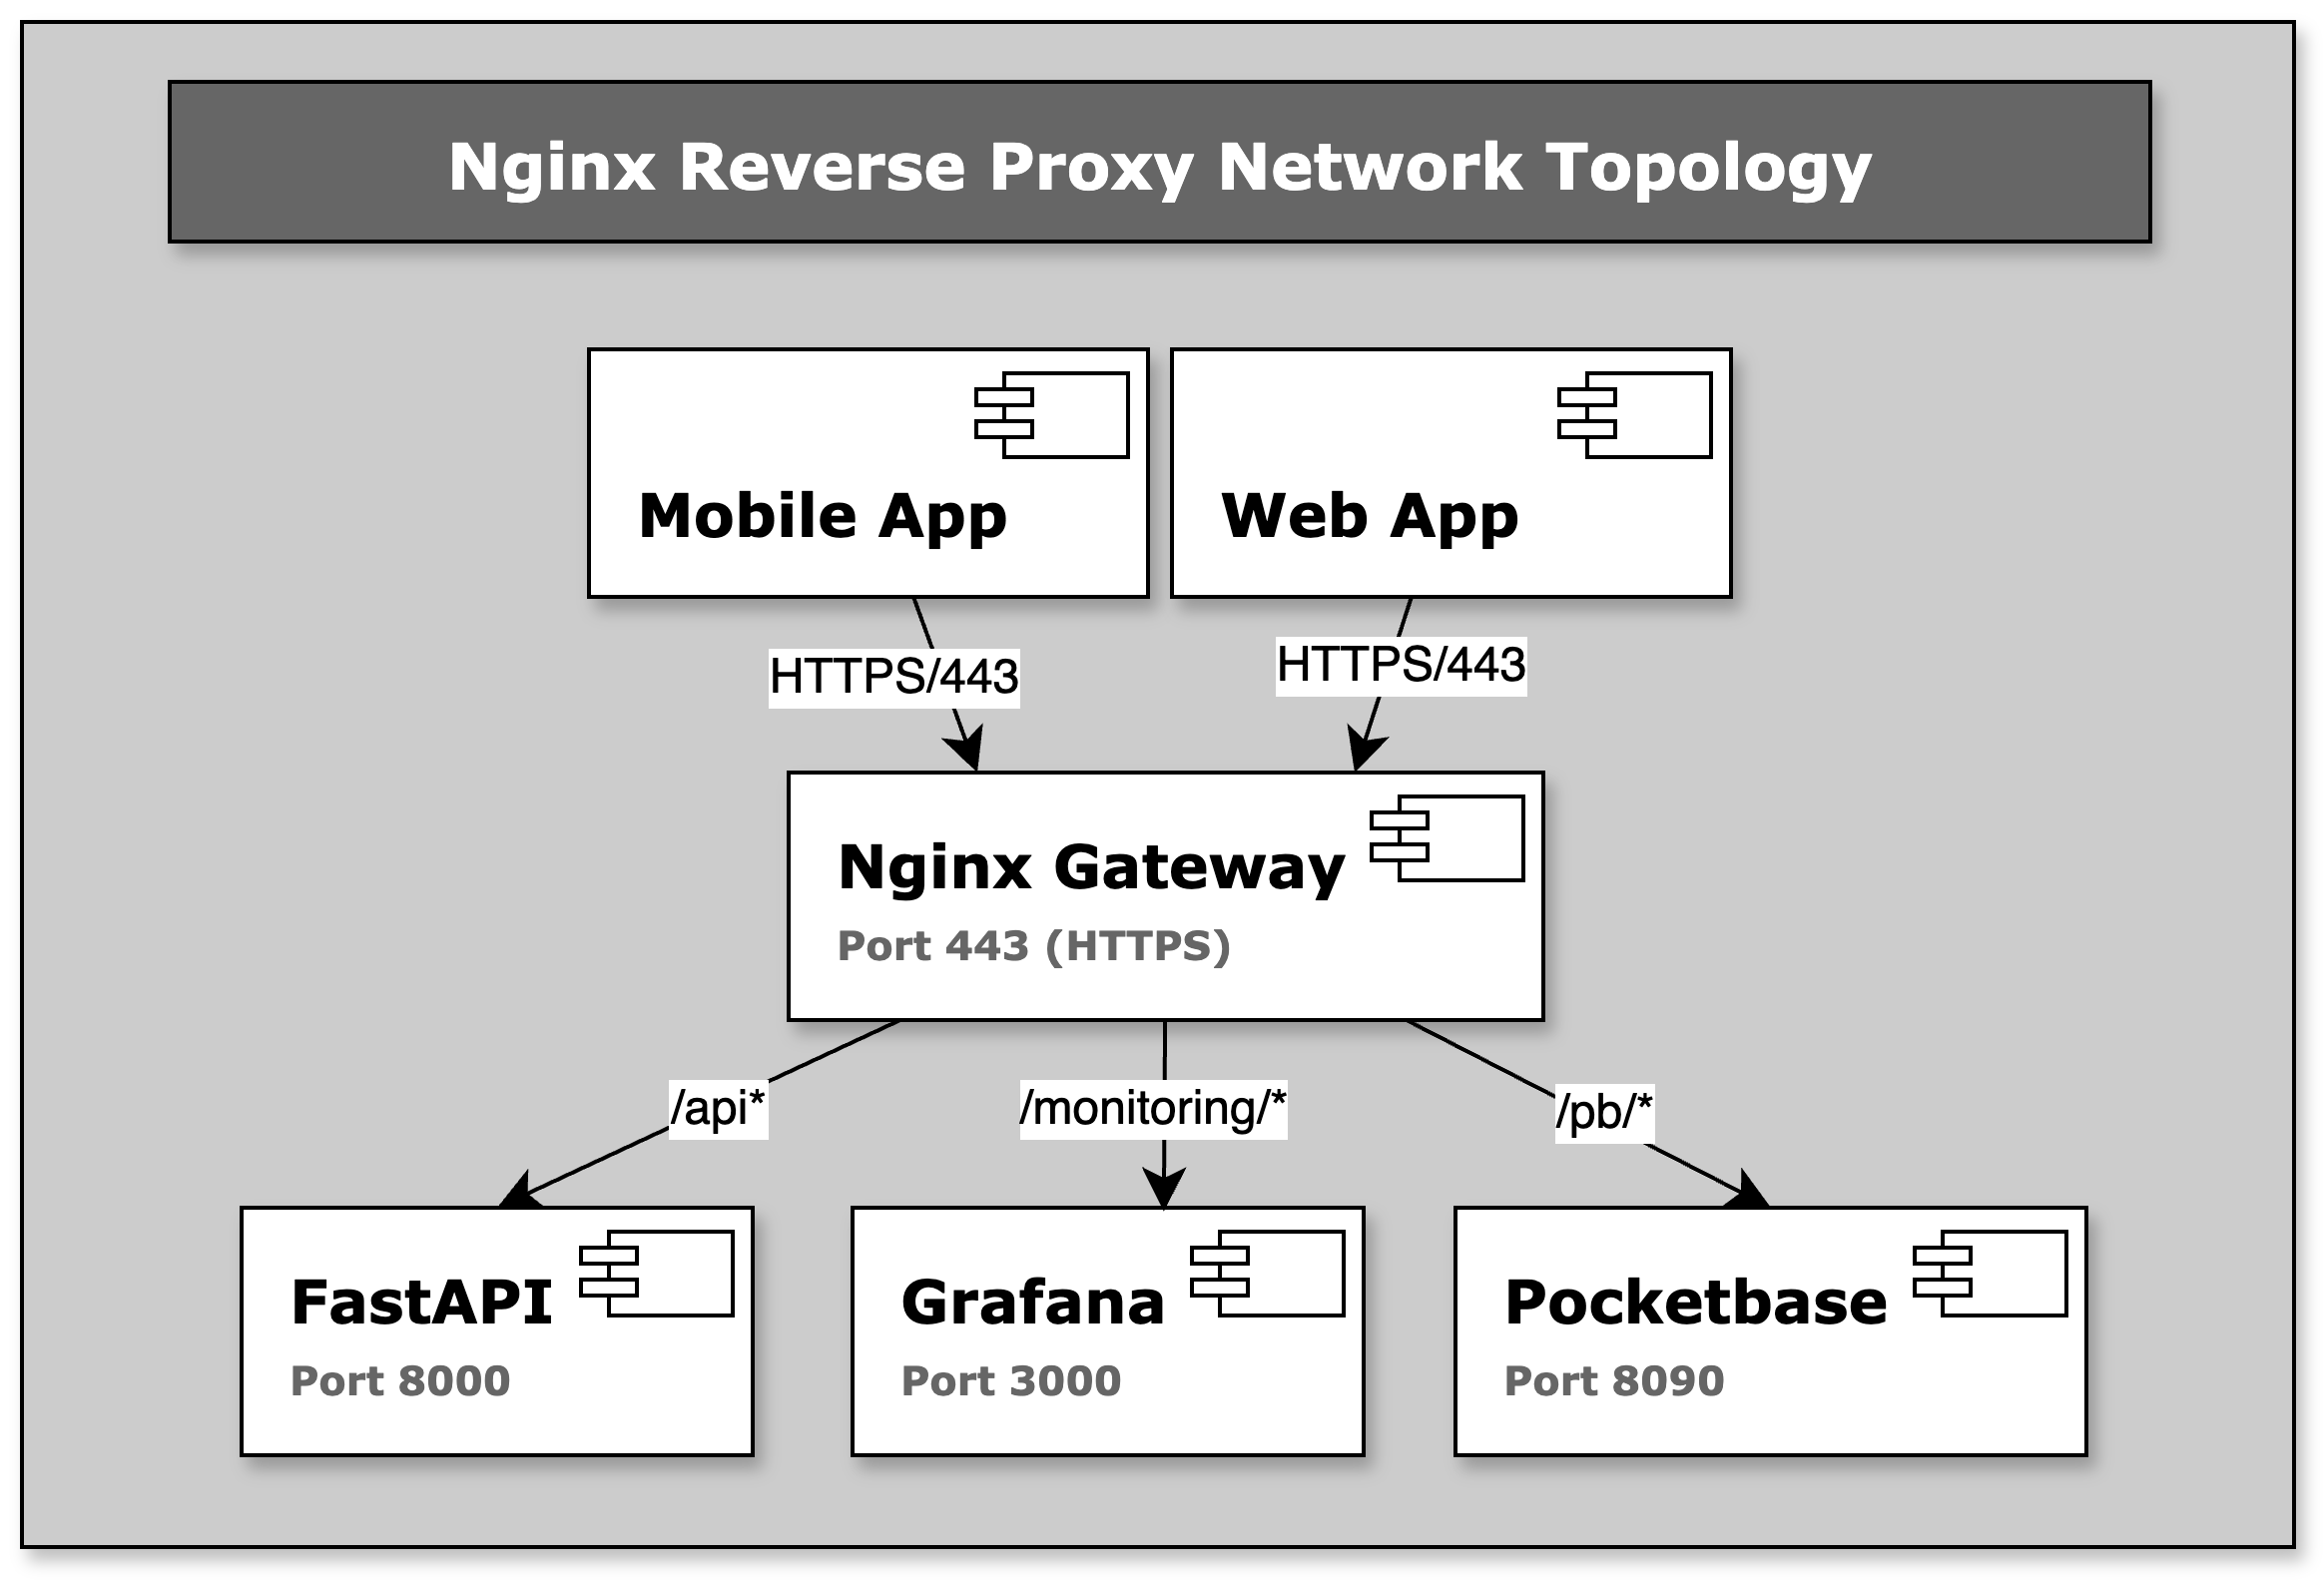
\includegraphics[width=0.5\textwidth]{figs/chapter4/network_topology.png}
    \caption[Network Topology Diagram]{Network topology diagram}
    \label{fig:network_topology}
\end{figure}

The reverse proxy enforces \ac{https} redirection with 301\footnote{\url{https://httpstatuses.com/301}} status codes for all \ac{http} requests, securing communication across the system. \ac{ssl} termination occurs at the gateway level, reducing computational overhead on backend services while preserving end-to-end encryption for client communications.

\subsubsection{Authentication Architecture} \label{subsubsection:auth_authorization}

The authentication architecture delegates token validation to the application layer while the gateway handles \ac{ssl} termination and security headers, including \ac{cors} configuration. The gateway does not perform token validation, preserving separation of concerns between infrastructure and application logic. At the application layer, input validation uses Pydantic\footnote{\url{https://docs.pydantic.dev/latest/}} models with email validation following RFC 5322\footnote{\url{https://datatracker.ietf.org/doc/html/rfc5322}} standards, alongside media type restrictions and size limits for file uploads.

\subsubsection{Rate Limiting and Throttling} \label{subsubsection:rate_limiting}

The Nginx configuration applies differentiated rate limiting based on endpoint functionality and security requirements. Considering system protection with standard application usage patterns, \ac{api} endpoints enforce 60 requests per minute with burst capacity of 20 requests. Authentication endpoints apply stricter limits of 10 requests per minute with 5-request bursts to prevent credential-based attacks, such as brute force attempts.

File upload functions receive 20 requests per minute with 10-request bursts, accounting for the time-intensive nature of image processing while preventing abuse. Administrative interfaces implement the most restrictive limits: 5 requests per minute with configurable burst capacity. The limits were designed to accommodate legitimate use cases incorporated in the application and to block abusive patterns. Table \ref{tab:rate_limiting_config} summarizes the complete rate limiting configuration across all endpoint types.

Connection limiting complements request rate limiting by restricting concurrent connections per \ac{ip} address. \ac{api} operations allow up to 10 concurrent connections per \ac{ip}. At the same time, authentication endpoints limit connections to 3 per \ac{ip}, preventing connection exhaustion attacks while accommodating legitimate multi-tab browsing and mobile application usage.

Rate limiting uses Nginx's \texttt{limit\_req} and \texttt{limit\_conn} modules with memory-based storage for fast enforcement without external dependencies. Rate limit violations return 429\footnote{\url{https://httpstatuses.com/429}} status codes with appropriate error messages, allowing client-side retry logic and clearly communicating the limitation to \ac{api} consumers. Figure \ref{fig:rate_limiting_effectiveness} demonstrates the effectiveness of these rate limiting measures in protecting the system from abusive traffic patterns.

\begin{table}[htbp]
    \centering
    \caption[Rate Limiting Configuration]{Rate limiting configuration by endpoint type with request limits and burst capacities}
    \label{tab:rate_limiting_config}
    \begin{tabular}{@{}llll@{}}
        \toprule
        \textbf{Endpoint Type} & \textbf{Rate Limit} & \textbf{Burst Capacity} & \textbf{Connection Limit} \\
        \midrule
        General \ac{api} & 60 requests/min & 20 requests & 10 connections \\
        Authentication & 10 requests/min & 5 requests & 3 connections \\
        File Upload & 20 requests/min & 10 requests & 5 connections \\
        PocketBase Admin & 5 requests/min & 3 requests & 2 connections \\
        Grafana Monitoring & 5 requests/min & 5 requests & 2 connections \\
        \bottomrule
    \end{tabular}
\end{table}

\begin{figure}[htbp]
    \centering
    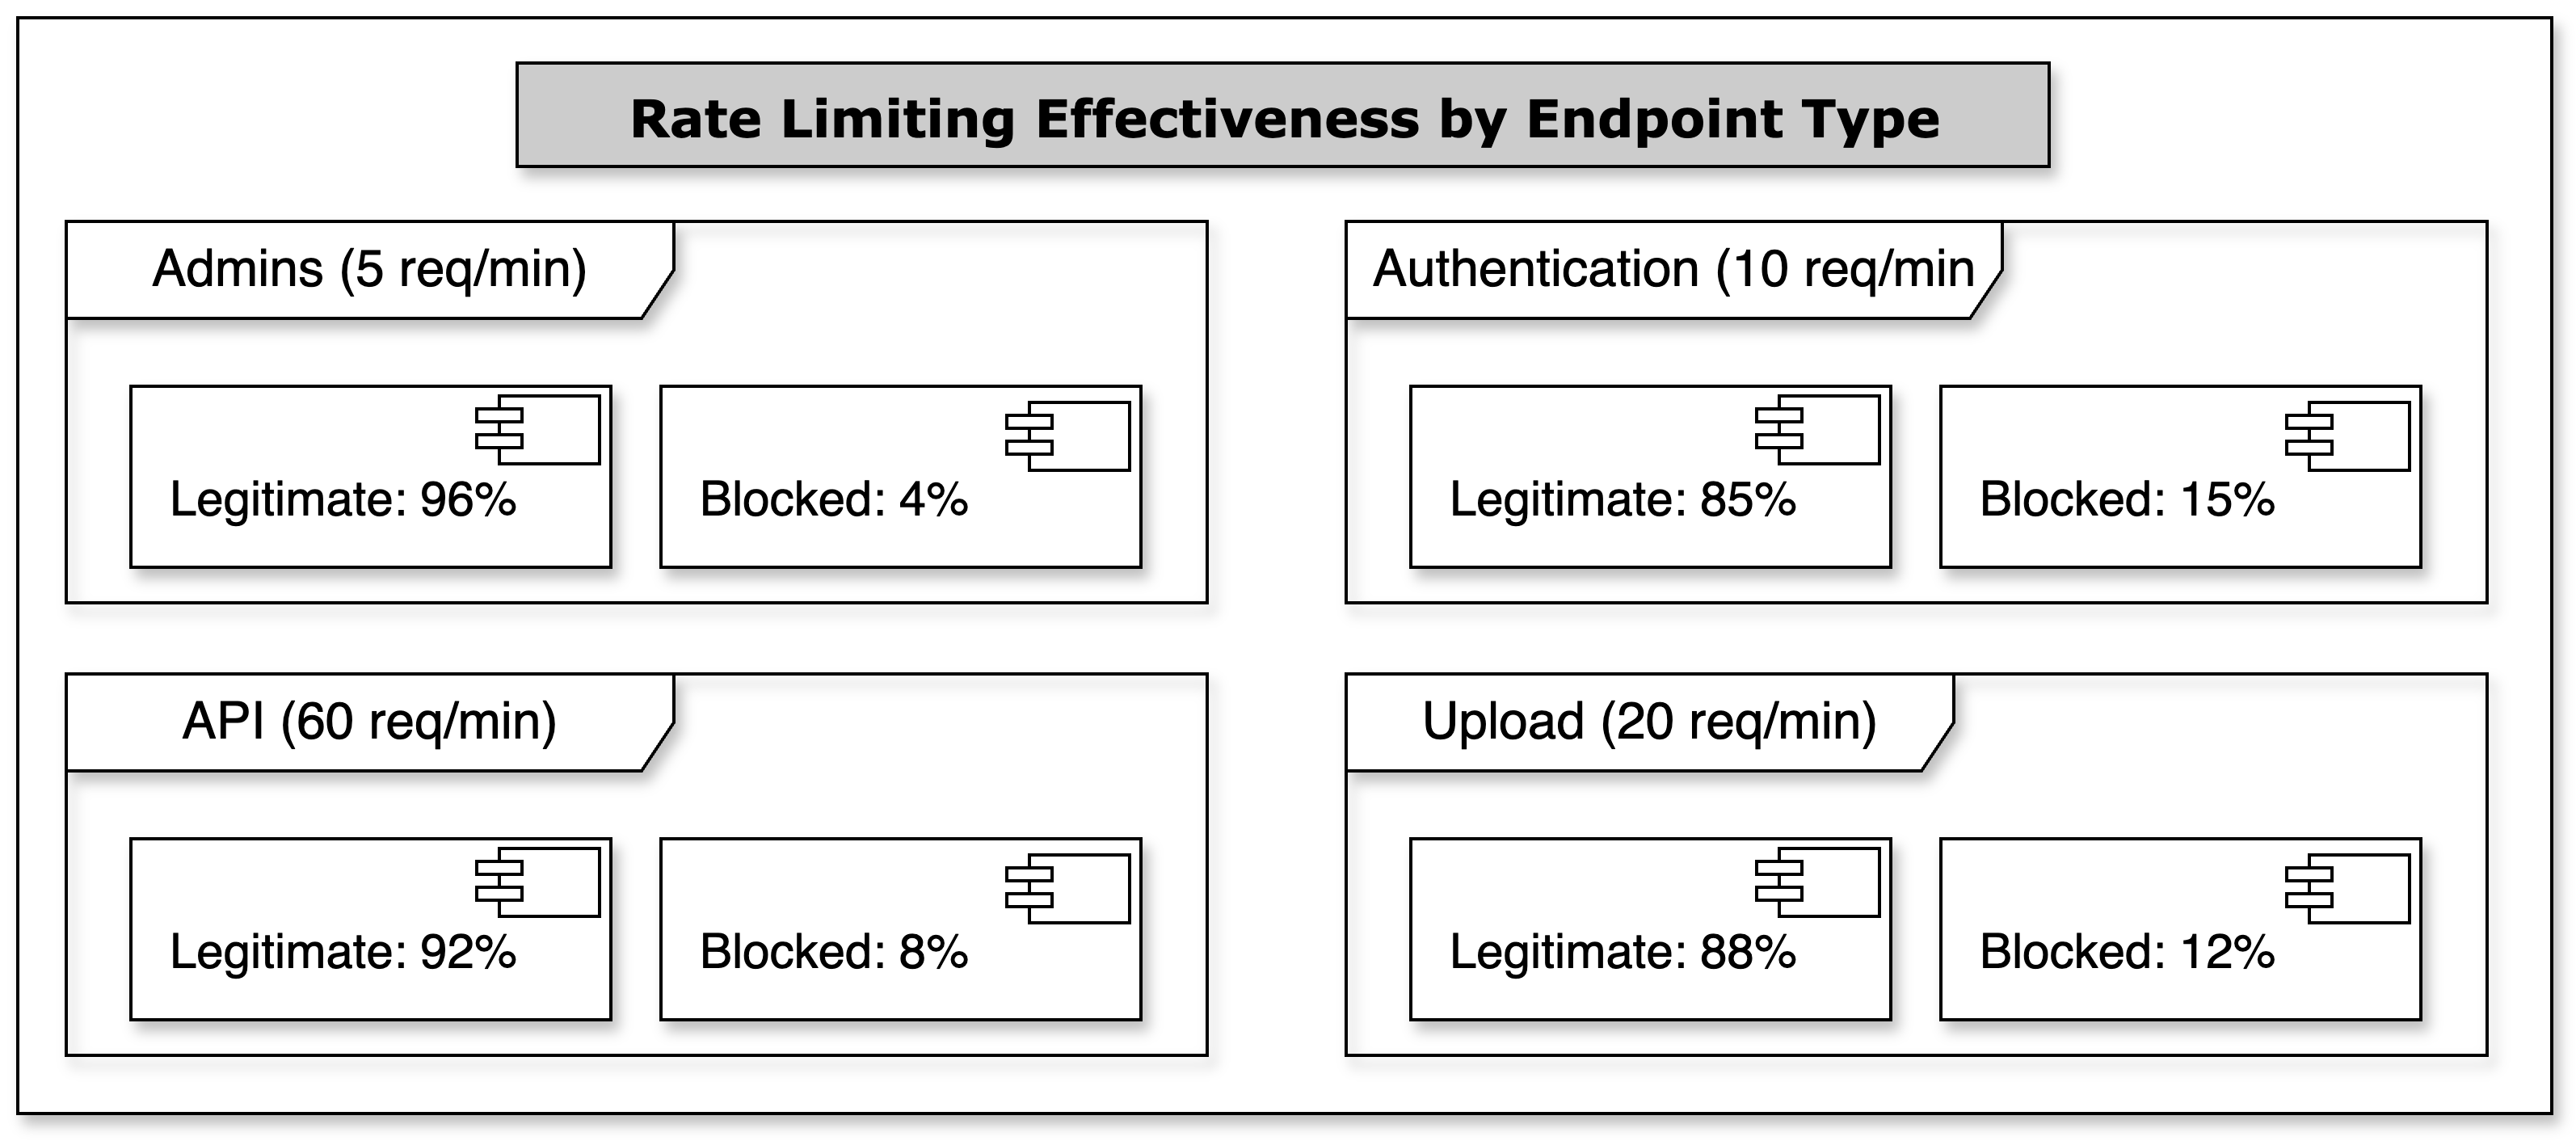
\includegraphics[width=0.75\textwidth]{figs/chapter4/rate_limiting_chart.png}
    \caption[Rate Limiting Effectiveness]{Rate limiting effectiveness metrics showing request blocking rates and system protection across different endpoint types}
    \label{fig:rate_limiting_effectiveness}
\end{figure}

\subsection{Community and Location Services} \label{subsection:community_location_services}

Community and location services establish the organisational foundation and geographic intelligence that enable multi-tenant operation and location-aware matching. The module manages hierarchical relationships between users, communities, and physical collection points while providing geographic calculations for proximity-based item matching.

\subsubsection{Community Management Architecture}

The community management system implements organisational control, handling the relationships and permissions that define the multi-tenant architecture. It provides role-aware access patterns where system administrators can manage their assigned communities with full administrative capabilities, local managers access communities through their associated managing points with operational permissions, and ordinary users participate in multiple communities based on their membership associations. Administrative operations support community configuration updates, including visual identity management through avatar uploads and ownership transfer with appropriate validation safeguards.

A dedicated service module manages user-community associations and handles the many-to-many relationships between ordinary users and their communities. The architecture enables efficient retrieval of all members within a specific community for administrative oversight, while also supporting user-centric queries to determine an individual's community memberships. The temporal dimension of these relationships is preserved through timestamp tracking, which is recorded when users join communities for audit and analysis purposes. The implementation uses database expansion capabilities to retrieve complete relationship graphs in a single operation, improving performance for organisational queries.

\subsubsection{Local Managing Points Implementation}

A specialised service manages physical collection and distribution points, combining location management with geospatial intelligence. When establishing new managing points, the system processes geographic coordinates as structured data containing precise latitude and longitude information, handles image uploads for visual identification of physical locations, and validates community associations to maintain proper organisational boundaries. The implementation supports flexible data retrieval with configurable pagination ranging from single-item queries to bulk operations processing up to 100,000 records. At the same time, relationship expansion capabilities allow selective loading of related data based on performance requirements.

Modification operations support partial updates to managing point configurations, enabling changes to geographic coordinates when facilities relocate and image updates for refreshed visual identification.

\subsubsection{Geographic Distance Calculations}

The location calculation service implements geographic algorithms that power the system's proximity-based matching capabilities. Distance calculations employ the Haversine formula \cite{Sinnott1984} to compute great circle distances between coordinate pairs, providing accurate measurements that account for the Earth's spherical geometry. Distance categorisation uses configurable thresholds that define proximity bands: very close for items within 1 kilometre, close for 5-kilometre ranges, moderate for 20-kilometre distances, and far for separations up to 100 kilometres.

Distance measurements are transformed into normalised proximity scores through a scaling algorithm that applies linear interpolation for nearby items and logarithmic decay for distant objects, making minor distance differences matter more for nearby items while still considering distant matches when relevant. The coordinate extraction system processes location data from multiple sources and formats, integrating geographic information into the \ac{ai} matching pipeline for location-aware item pairing decisions.


% ____________________ AI Integration and Matching Implementation ____________________ %

\section{\ac{ai} Integration and Matching Implementation} \label{section:ai_integration}

\ac{ai} integration enables multimodal analysis for automated item matching using \ac{llava}-powered visual and textual comparison with scoring algorithms. Multi-factor scoring combines with confidence thresholds to identify potential matches.

\subsection{\ac{llava} Client Implementation} \label{subsection:llava_client}

The \ac{llava} client provides multimodal \ac{ai} capabilities through integration with Ollama server infrastructure, combining text and image analysis for automated item description generation and visual similarity matching. The client connects to the remote Ollama server using Bearer token authentication with \ac{jwt} format credentials, with the implementation requiring critical fixes during development to transition from broken \texttt{ollama.generate} imports to proper \texttt{ollama.Client()} instantiation with correct authentication headers.


The client configuration includes host specification via environment variables, authorisation headers for secure communication, and connection parameters configured for different analysis types. Text analysis uses a 2048 token context with 30-second timeouts and a temperature of 0.1 for consistent results, while image analysis extends to a 4096 token context with 45-second timeouts to accommodate visual processing requirements.

The image processing service coordinates \ac{ai}-powered image analysis using the prompt "Describe the main central object in this image..." for automatic description generation. Category assignment operates through object matching against the complete classification taxonomy, with fallback to a general category when classification confidence proves insufficient. Image processing includes PNG\footnote{\url{https://en.wikipedia.org/wiki/Portable_Network_Graphics}} conversion and validation for \ac{ai} compatibility, creating consistent input formats for reliable analysis. The service uses batch file operations to improve performance during multiple image retrievals, while validation error handling prevents system interruptions when \ac{ai} services become temporarily unavailable.

\subsection{Matching Algorithm Implementation} \label{subsection:matching_algorithm}

The matching algorithm uses a multi-factor scoring system that combines semantic understanding, visual analysis, geographic and temporal proximity, and contextual relevance to identify potential item matches through \ac{ai}-powered comparison across multiple dimensions while maintaining performance characteristics necessary for real-time operation. The confidence calculation uses a calibrated weighted algorithm that balances different matching factors based on their empirical predictive value.

Description similarity represents the most significant factor at 40\% weight, utilising semantic text analysis to understand meaning beyond simple keyword matching. Category alignment contributes 25\% to the overall score, recognising that correct classification provides strong correlation signals. Visual similarity through multimodal image comparison accounts for 20\% of the score, providing crucial confirmation when textual descriptions may vary. Geographic proximity adds 10\% weight to favour nearby matches while still considering distant possibilities, and temporal relevance contributes the final 5\% to acknowledge the correlation between report and discovery timing.

The scoring architecture normalises each factor to a standard 0.0 to 1.0 scale before applying weights, creating balanced contributions regardless of underlying measurement scales. Figure \ref{fig:ai_scoring_system} illustrates the distribution of weighted scoring factors and the binary confidence threshold system that determines user interactions.

\begin{figure}[htbp]
    \centering
    \begin{subfigure}[t]{0.48\textwidth}
        \centering
        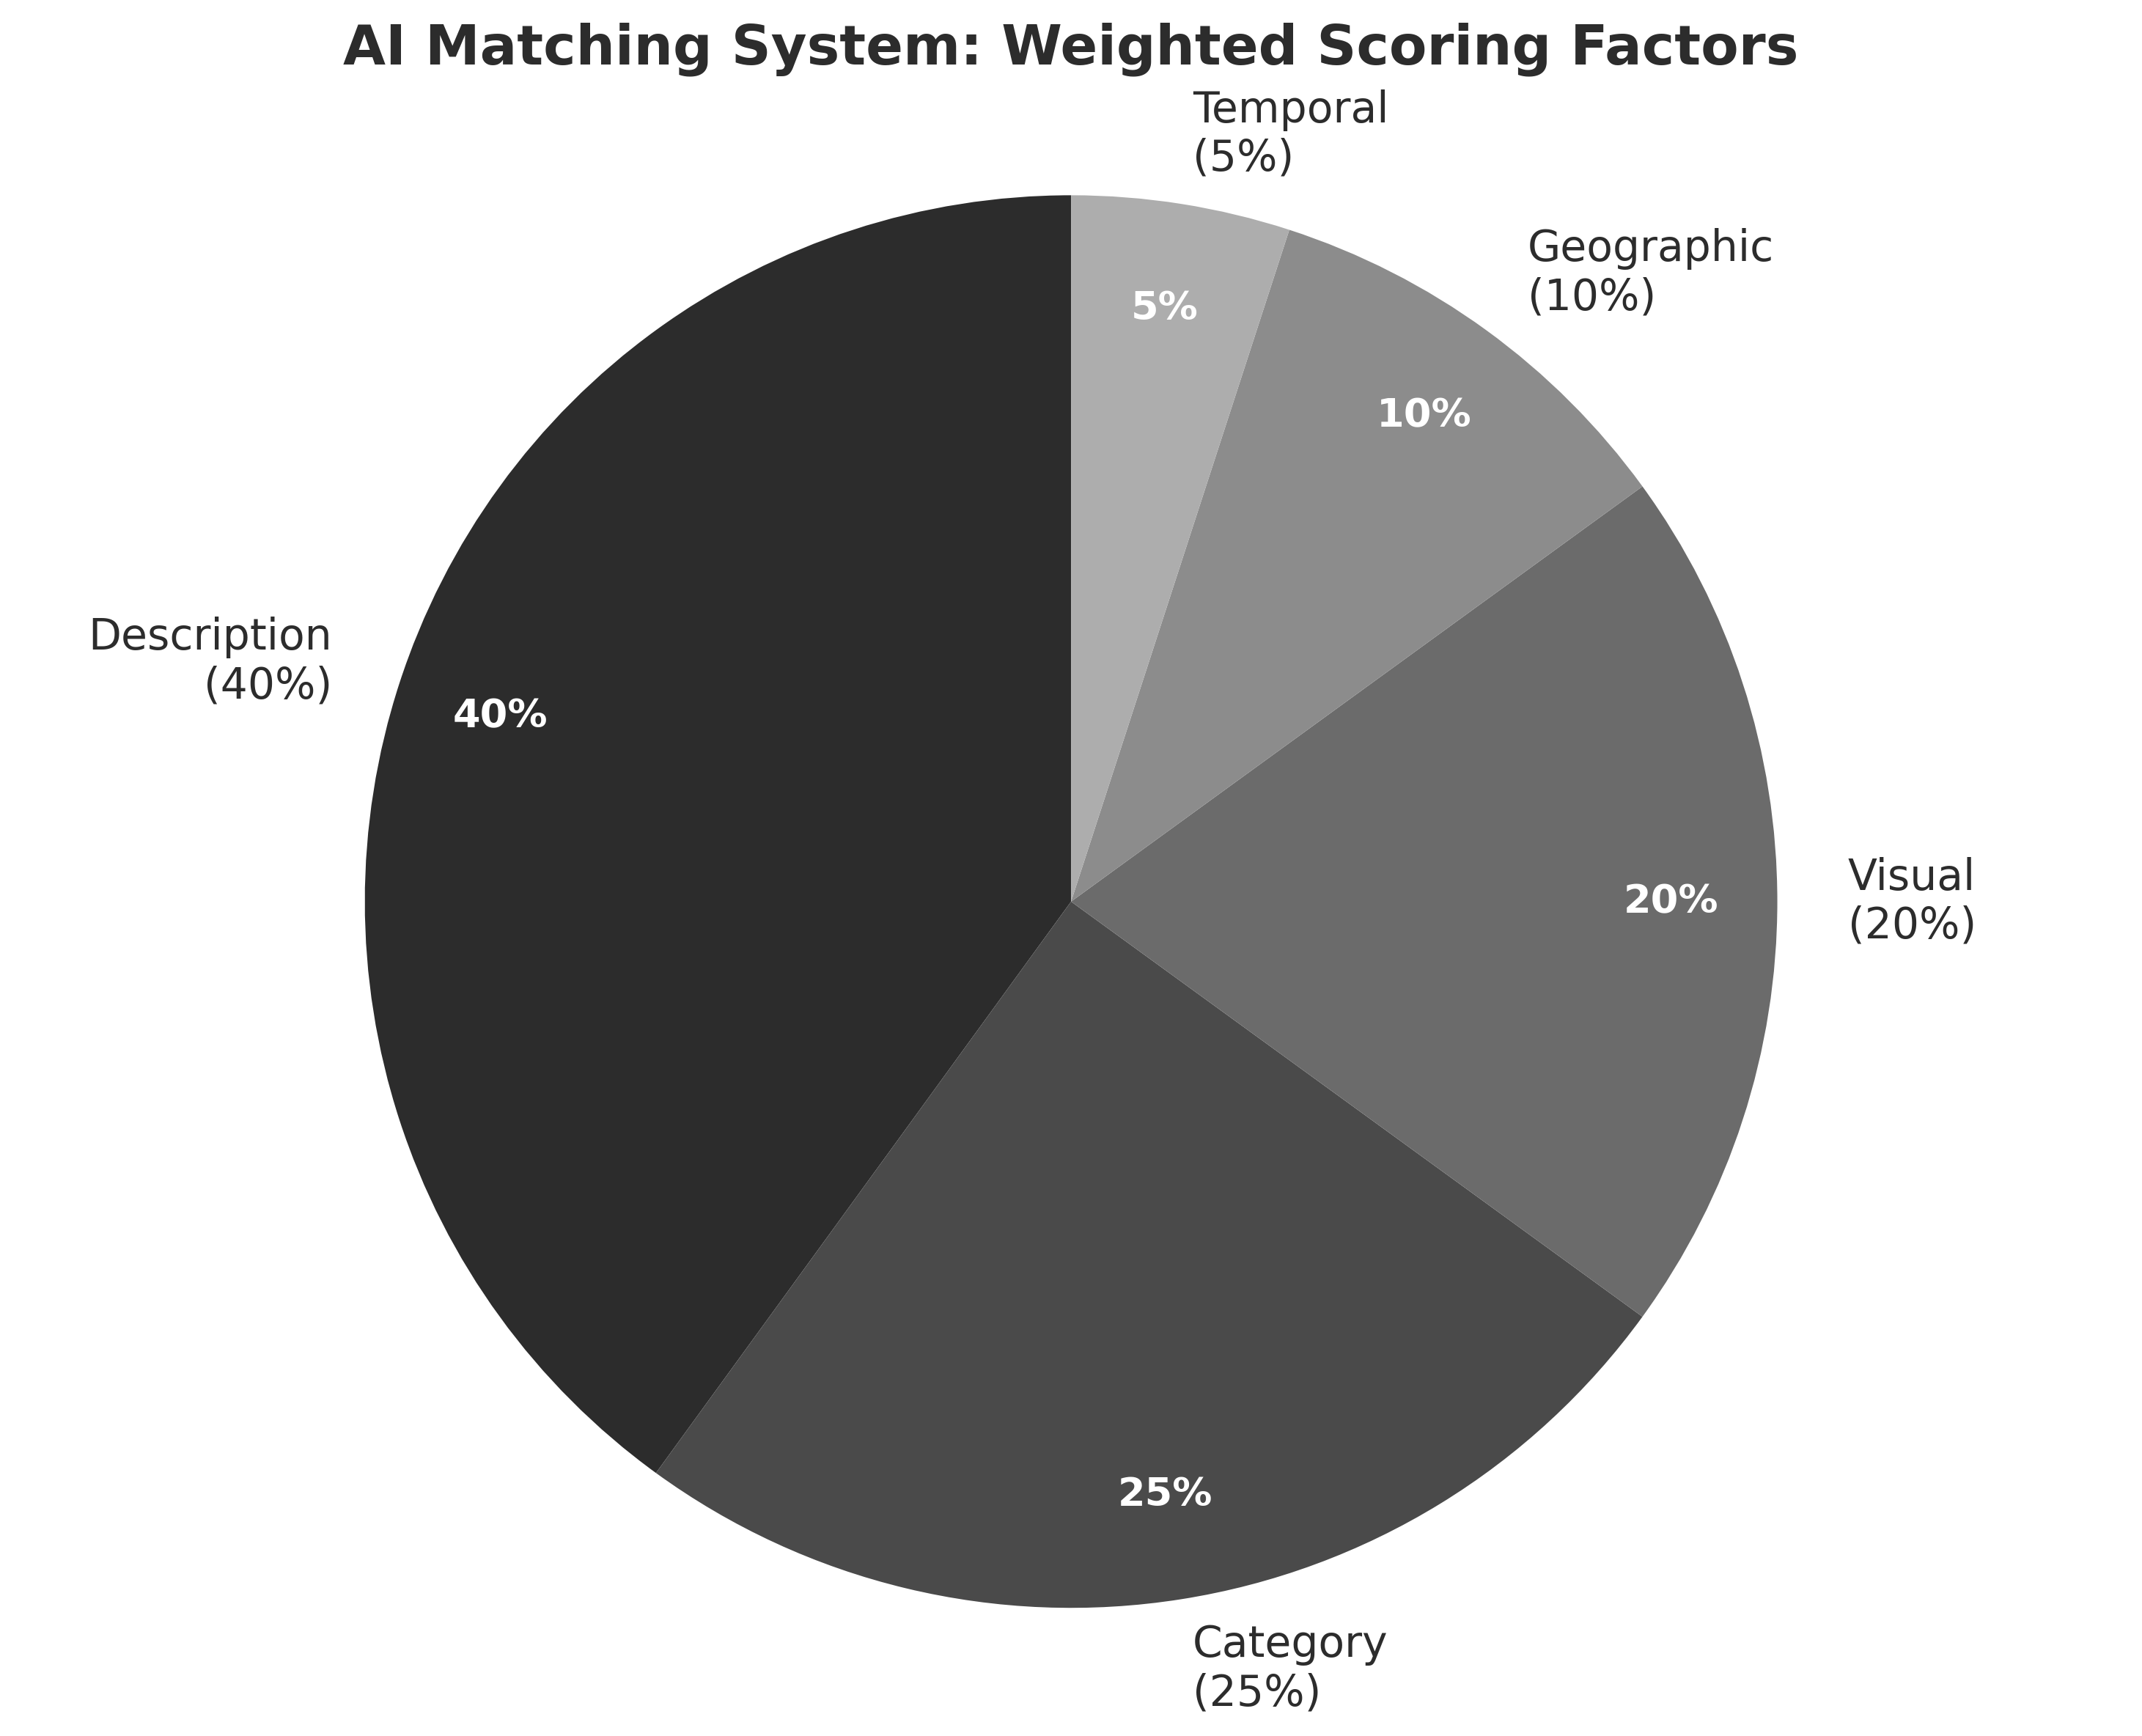
\includegraphics[width=\textwidth]{figs/chapter4/scoring_factors_chart.png}
        \caption{Weighted scoring factors distribution}
        \label{fig:scoring_factors}
    \end{subfigure}
    \hfill
    \begin{subfigure}[t]{0.48\textwidth}
        \centering
        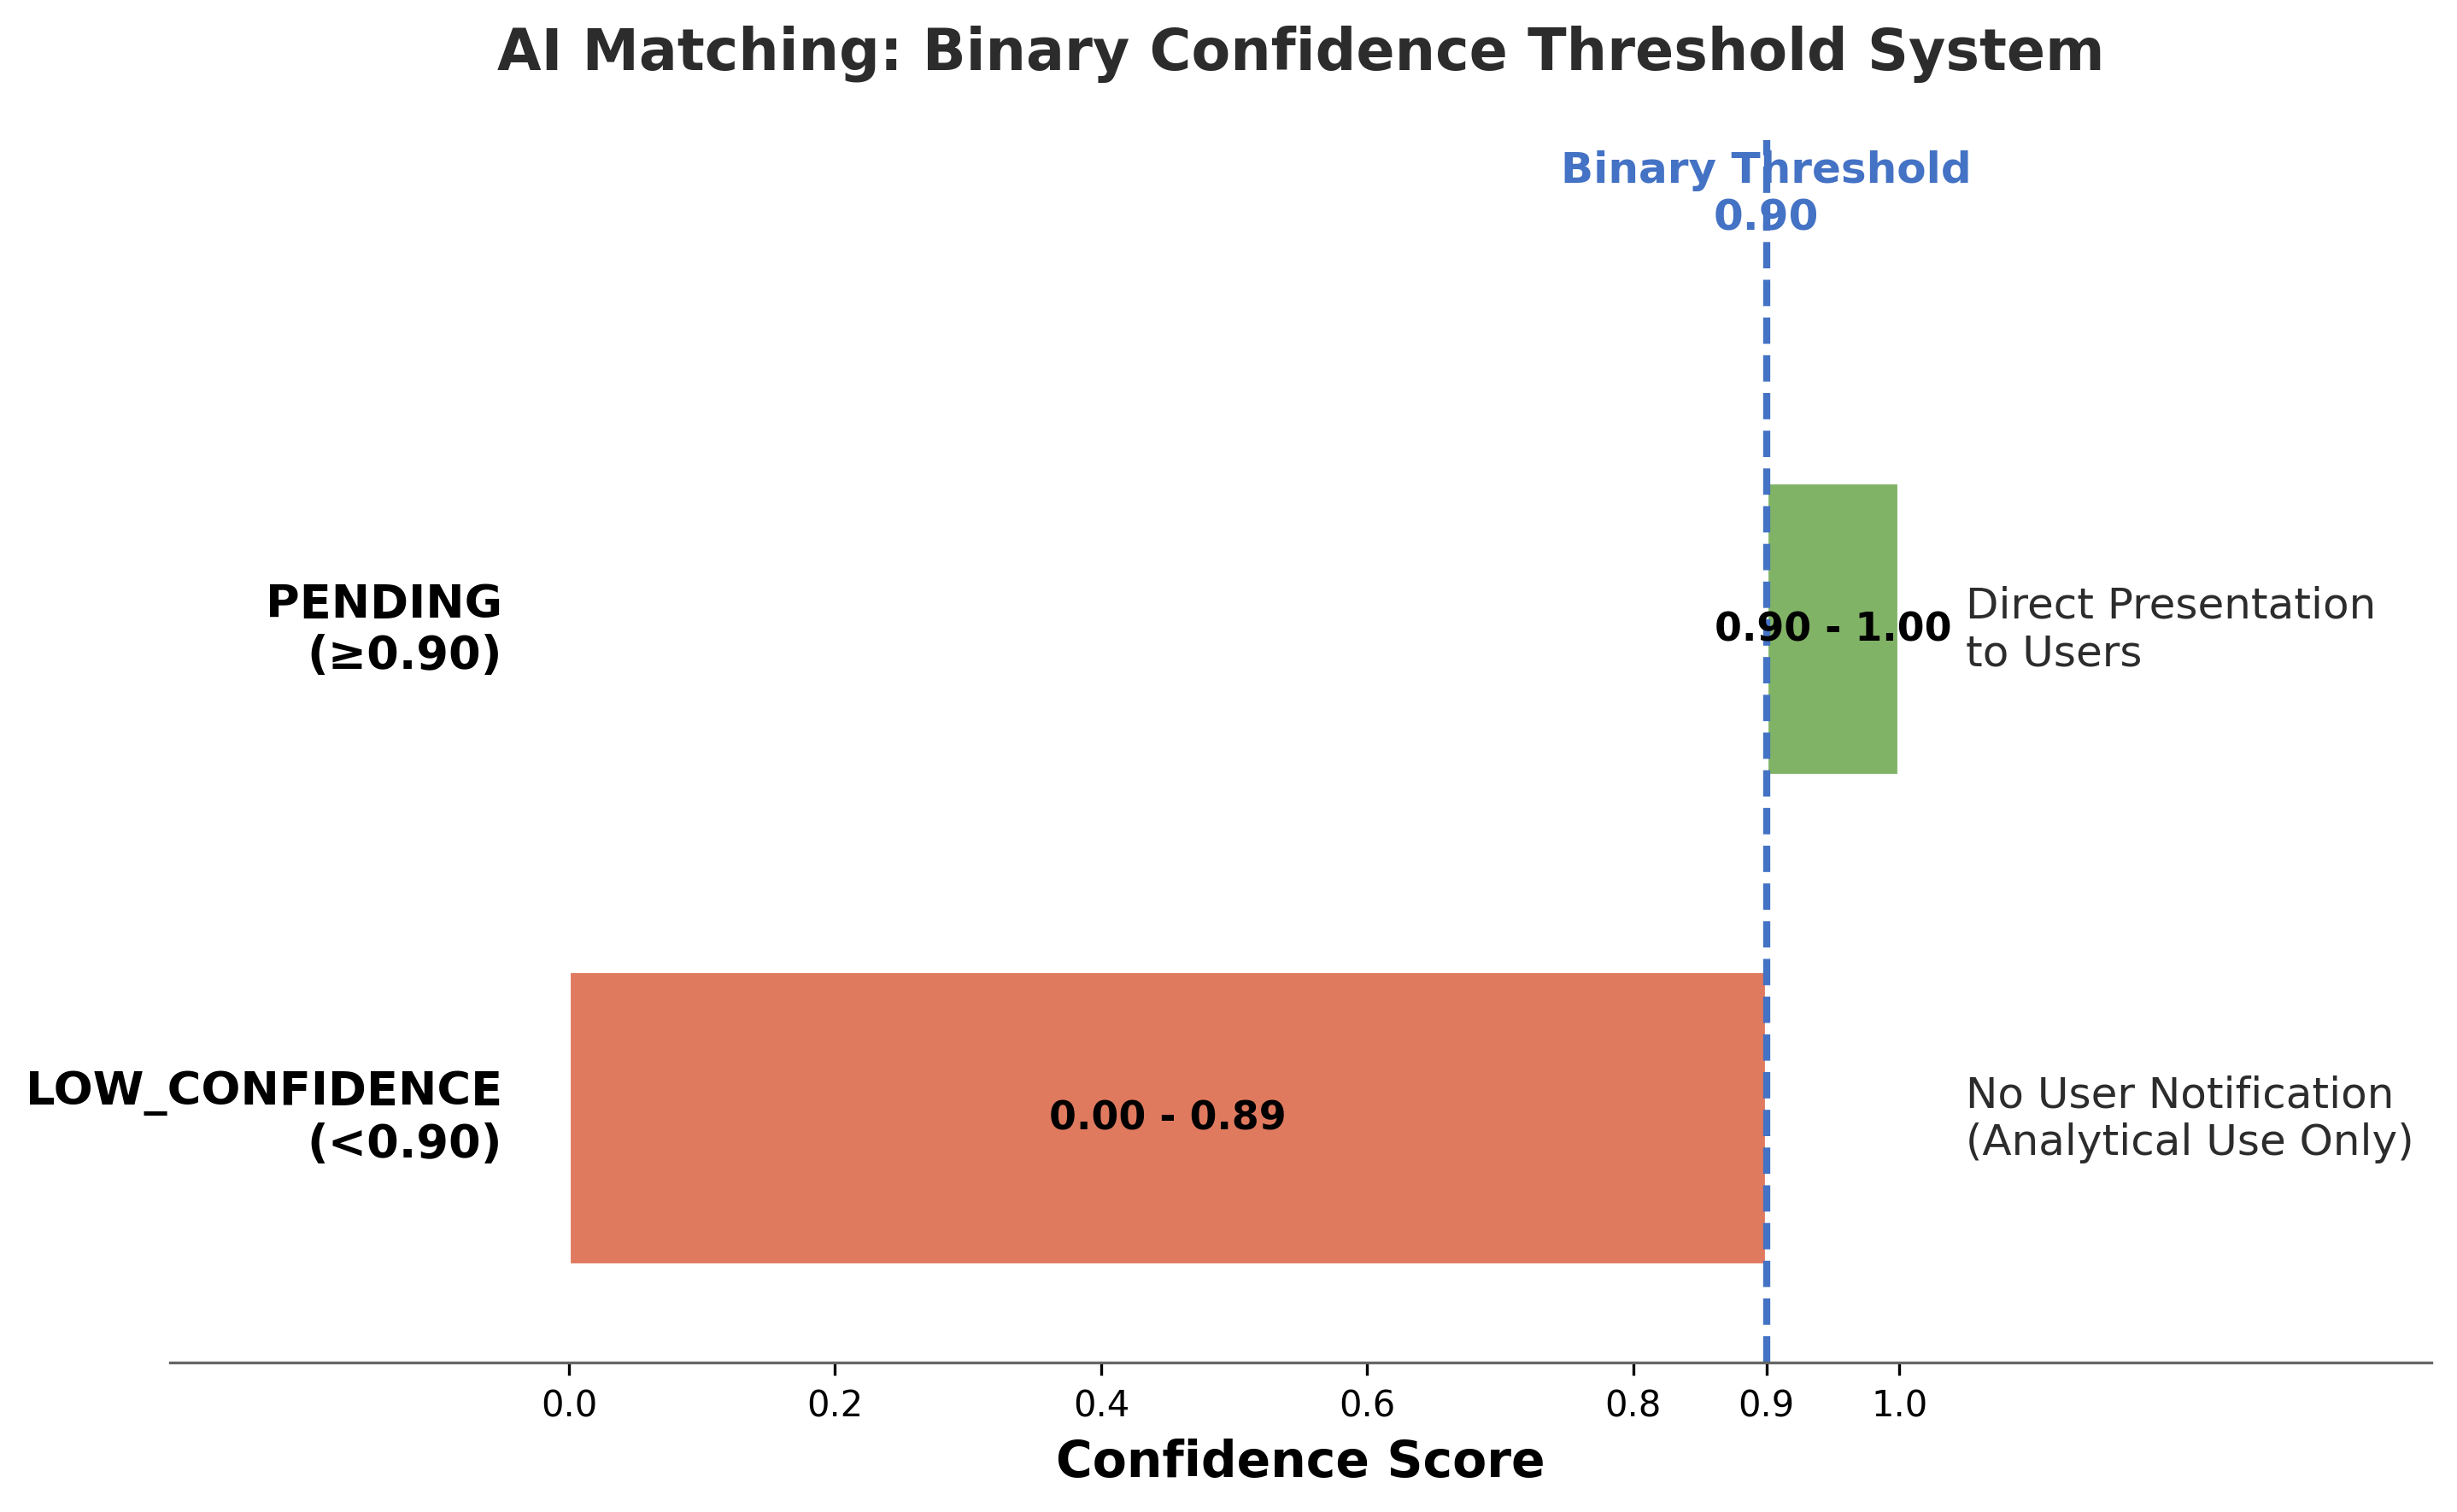
\includegraphics[width=\textwidth]{figs/chapter4/confidence_bands_chart.png}
        \caption{Binary confidence threshold and user interactions}
        \label{fig:confidence_bands}
    \end{subfigure}
    \caption{Scoring system}
    \label{fig:ai_scoring_system}
\end{figure}

A binary confidence threshold at 0.90 determines how users interact with potential matches. Matches achieving confidence scores at or above 0.90 are classified as \texttt{PENDING} status and presented to users as highly probable reunifications, requiring only minimal verification before confirmation. Matches scoring below 0.90 are classified as \texttt{LOW\_CONFIDENCE} status and are excluded from immediate user notification to prevent notification fatigue, though the system retains these matches for analytical purposes and algorithm improvement. The binary threshold system balances maximising successful reunifications while minimising false positive notifications that could undermine user trust, establishing clear operational boundaries and reducing complexity in both implementation and user experience.



\subsection{Queue Processing Implementation} \label{subsection:queue_processing}

Queue processing manages asynchronous item operations through a service-oriented architecture that balances continuous background processing and batch operations. A facade pattern coordinates four specialised services, each designed for specific operational requirements. Continuous processing maintains persistent background operations with sleep and backoff mechanisms that adapt to workload variations, maximising throughput by maintaining constant operation with minimal idle time. Batch processing manages community-specific operations with configurable batch sizes that balance throughput and resource utilisation. Administrative capabilities allow queue manipulation and manual intervention when necessary, prioritising reliability and data consistency over raw performance. Real-time monitoring provides statistics and health assessments for operational decisions and capacity planning.

Batch processing groups items by community for fair resource allocation across the multi-tenant architecture, with processing cycles handling up to 10 items per community. Adaptive timing uses 5-second delays between active processing cycles to prevent resource exhaustion, extending to 30-second idle periods when queues are empty to reduce computational overhead. Workflow management tracks item progression through clearly defined states that allow precise monitoring and error recovery. Items enter the queue in a pending state awaiting their processing turn, with the processing state indicating active \ac{ai} analysis in progress to prevent duplicate processing attempts. Completed and failed states represent terminal conditions that trigger appropriate follow-up actions, with state transitions using atomic operations wherever the underlying database supports them, supplemented by compensating actions for multi-step processes that cannot be completed atomically within the database's transactional constraints.

The queue system also distinguishes between transient and permanent failures with appropriate recovery strategies. Transient failures trigger exponential backoff retry mechanisms with gradually increasing delay intervals, while permanent failures are immediately marked and removed from active processing to prevent queue blockage. State tracking with unique identifiers and timestamps prevents duplicate processing during system restarts, allowing operations to resume exactly where interruptions occurred.

The monitoring infrastructure provides real-time visibility into queue operations through detailed metrics collection, tracking throughput with community-level granularity, latency across different processing stages, and success rates broken down by community and item type. The monitoring implementation integrates with Prometheus and Grafana for metrics collection, visualisation, and alerting capabilities, automatically tracking request latency, response patterns, and system resource utilisation with configurable alerting for threshold violations.

The matching algorithm performance analysis shows distinct characteristics between high-confidence and low-confidence matches. Figure \ref{fig:ai_matching_system} demonstrates the accuracy rates achieved for each confidence level and shows the corresponding processing time requirements.

\begin{figure}[htbp]
    \centering
    \begin{subfigure}[t]{0.48\textwidth}
        \centering
        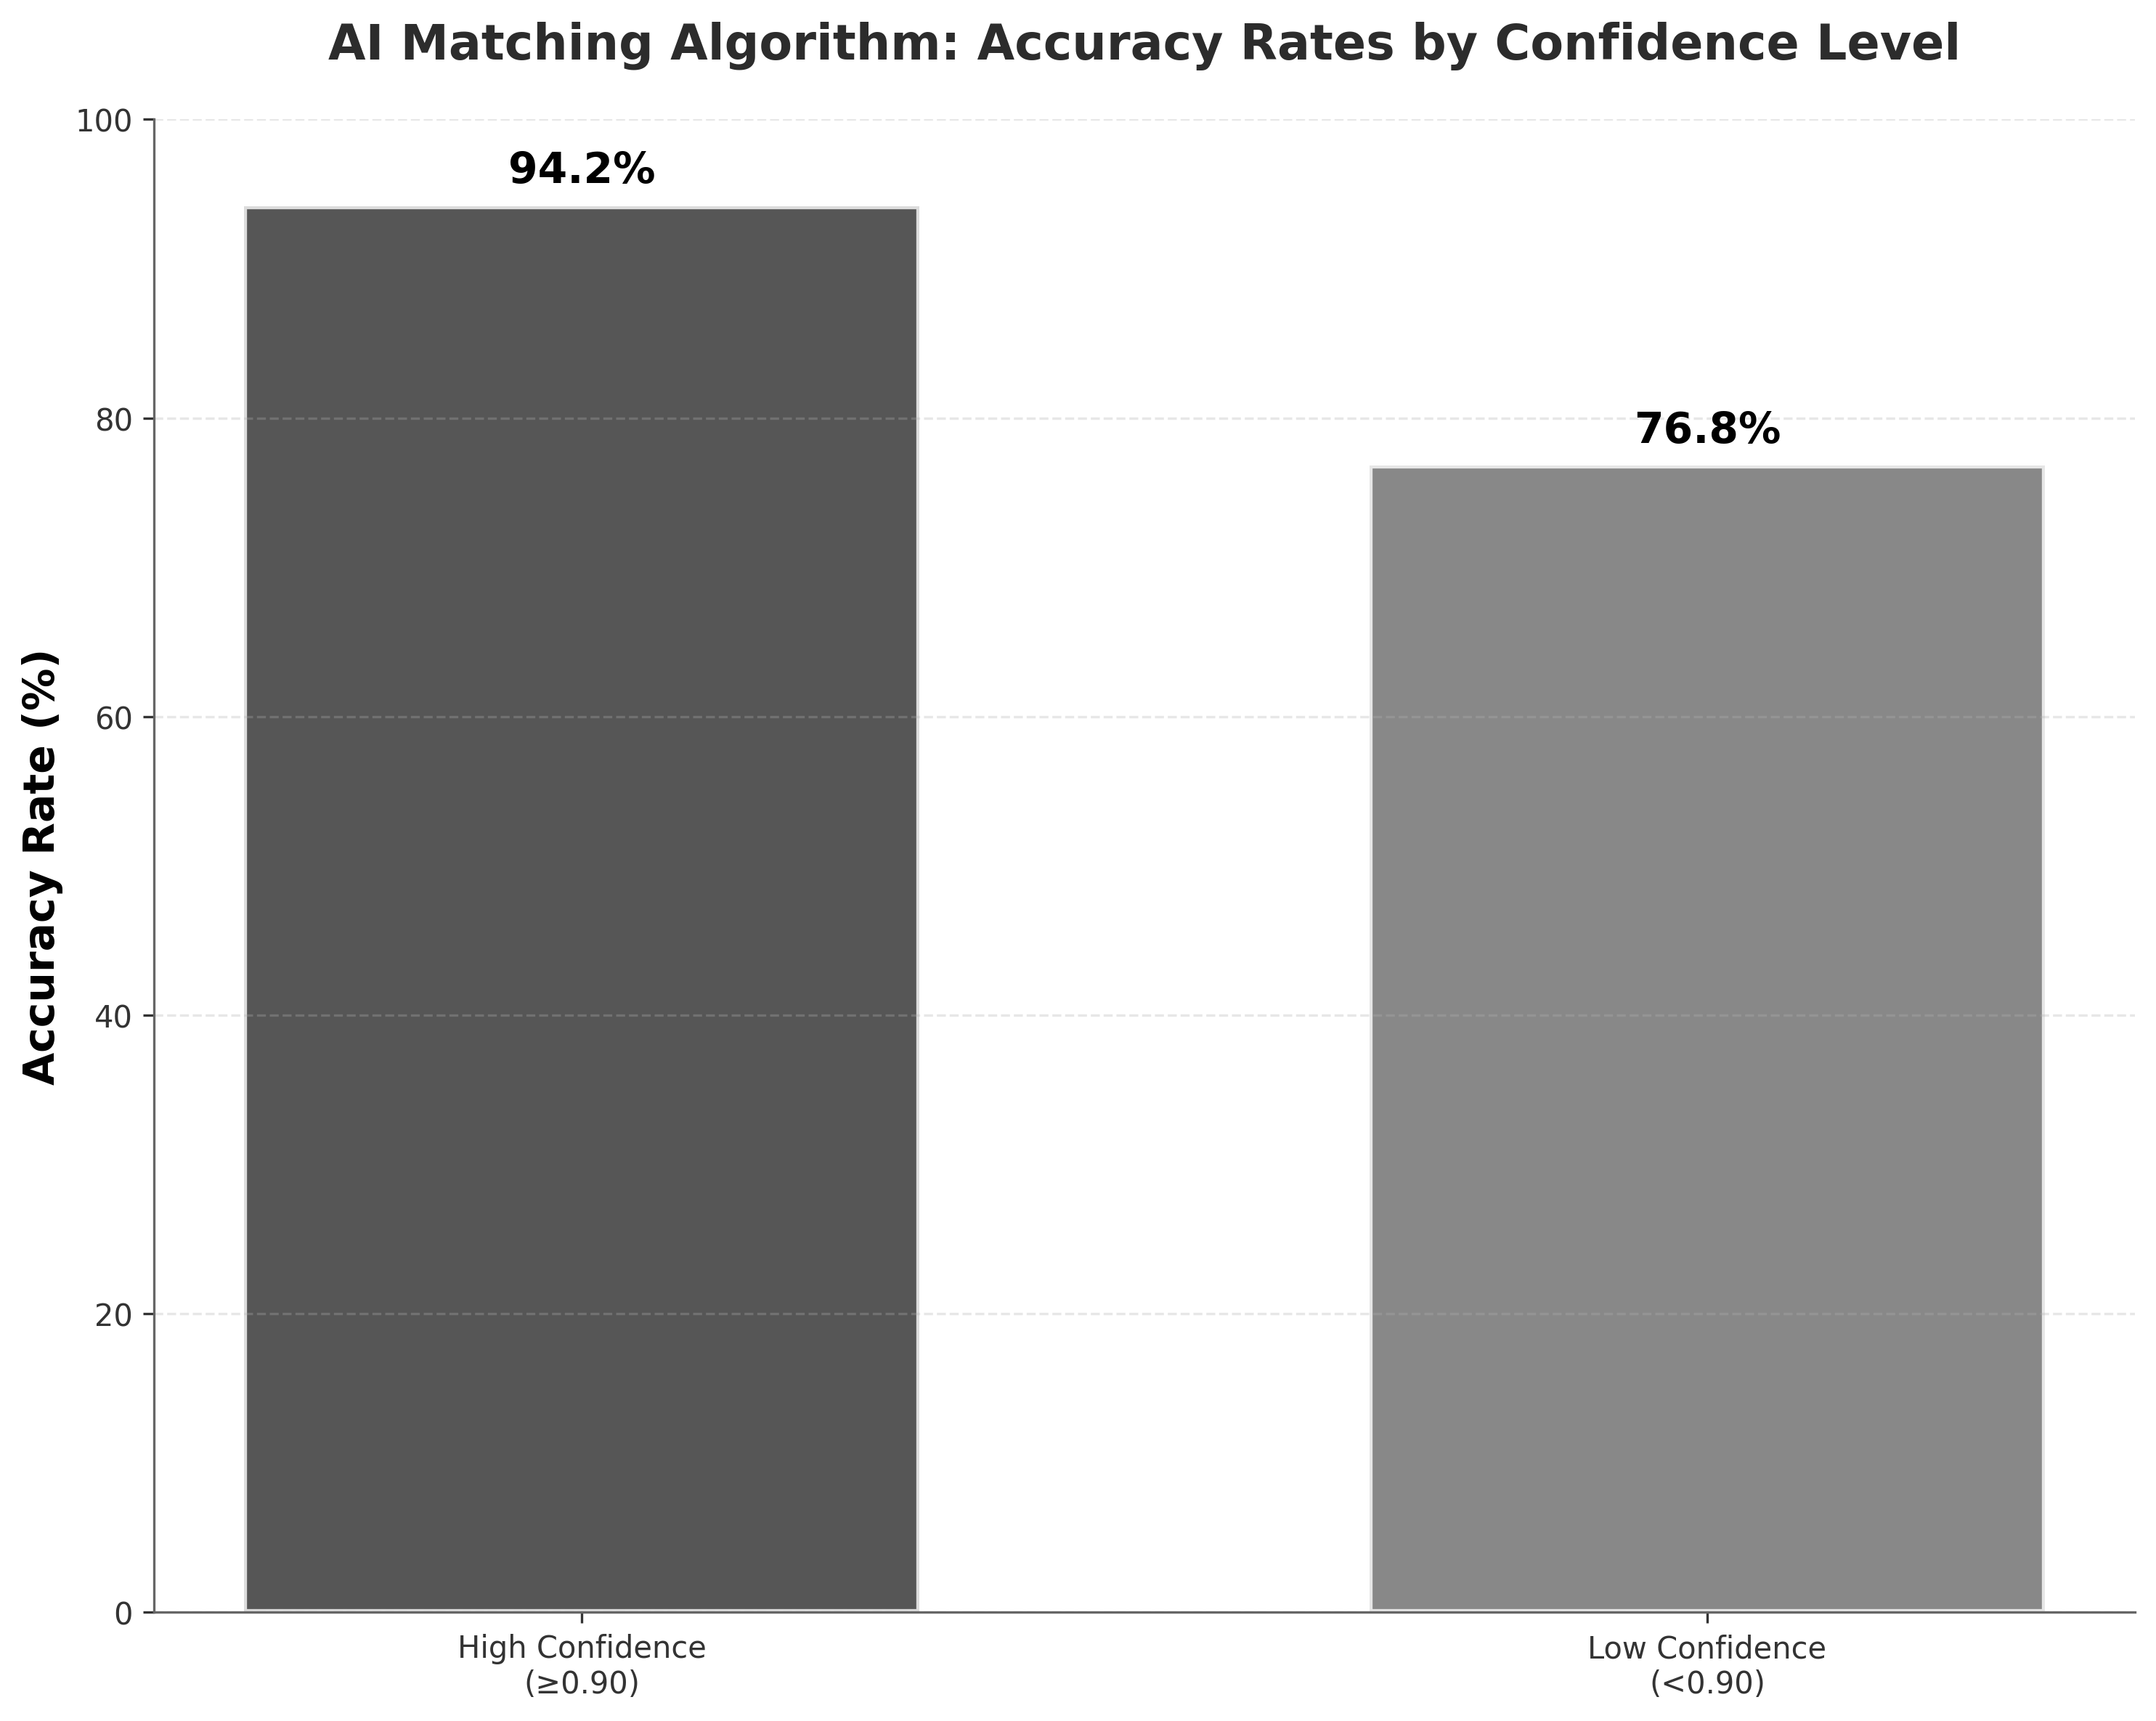
\includegraphics[width=\textwidth]{figs/chapter4/ai_accuracy_rates.png}
        \caption{Accuracy Rates by Confidence Level}
        \label{fig:ai_accuracy}
    \end{subfigure}
    \hfill
    \begin{subfigure}[t]{0.48\textwidth}
        \centering
        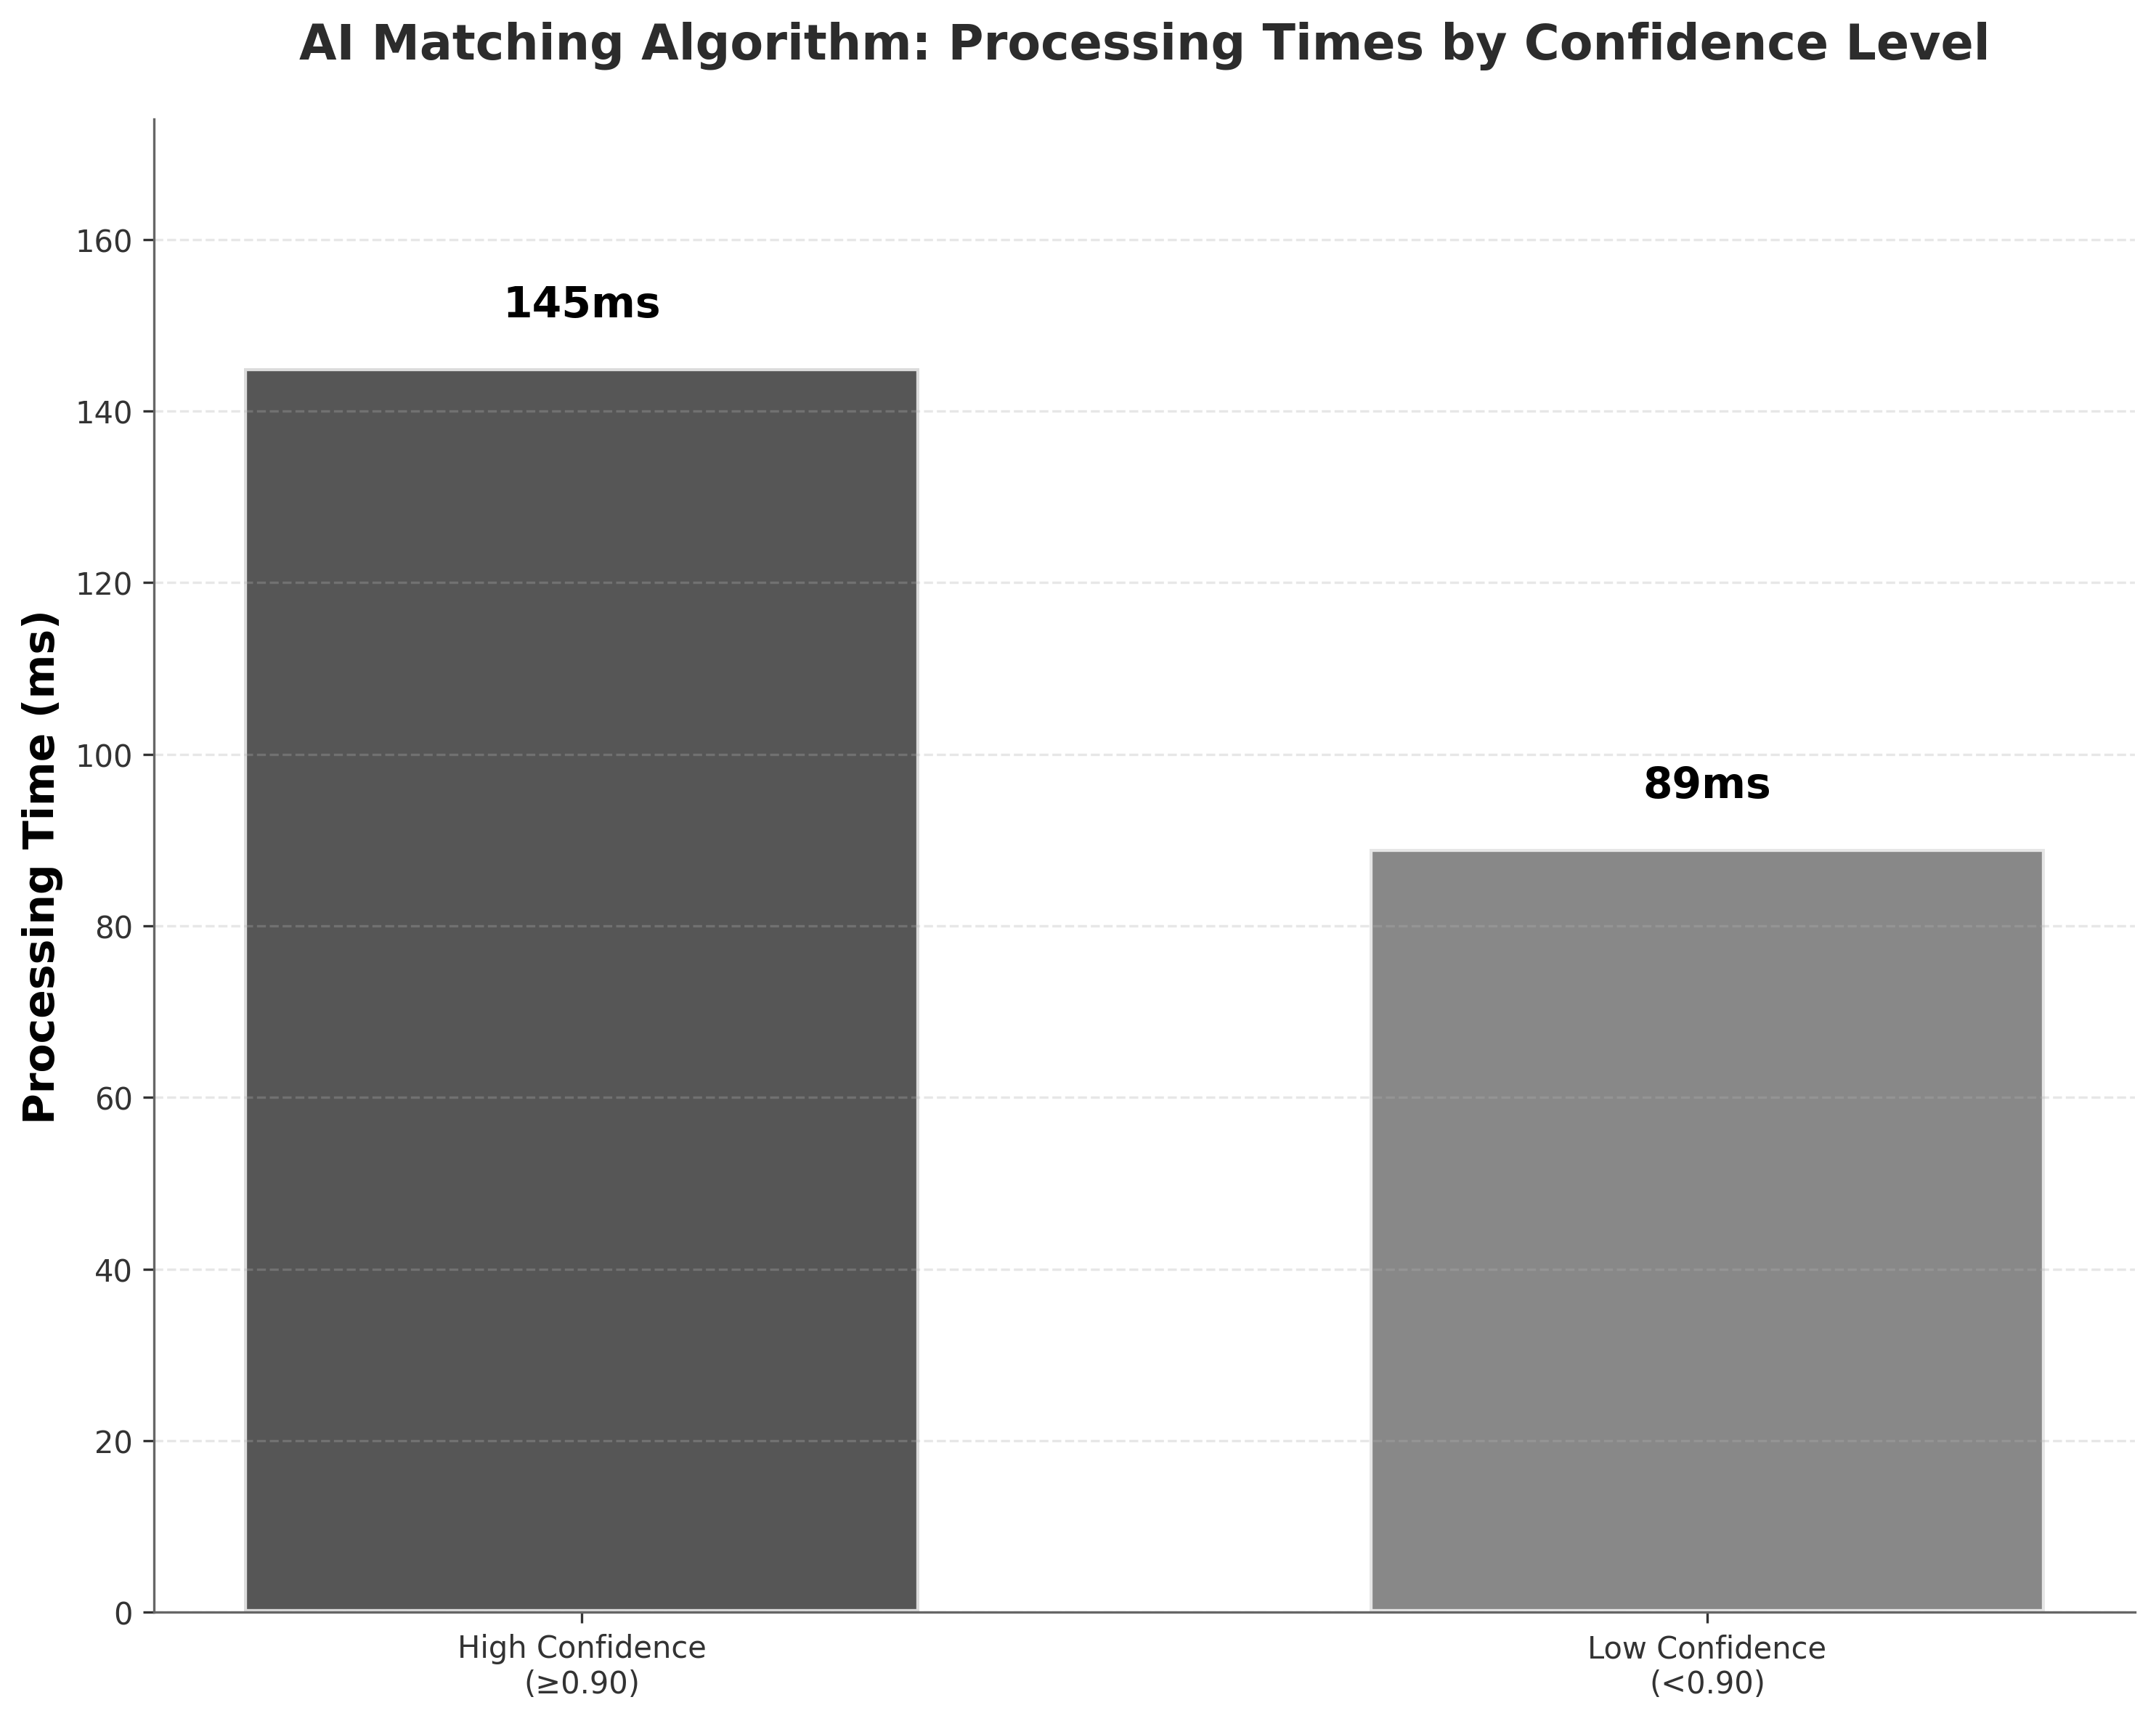
\includegraphics[width=\textwidth]{figs/chapter4/ai_processing_times.png}
        \caption{Processing Times by Confidence Level}
        \label{fig:ai_processing}
    \end{subfigure}
    \caption{AI Matching Algorithm Performance Metrics}
    \label{fig:ai_matching_system}
\end{figure}

% TODO: Add sample Grafana dashboard screenshots showing queue monitoring metrics, system health panels, and alert configurations

% ____________________ Frontend Interfaces ____________________ %

\section{Frontend Interfaces} \label{section:frontend_interfaces}

Two distinct user interfaces are tailored to different user roles and operational contexts. The web application provides dashboard capabilities for local managers and administrators, and the mobile application enables ordinary users to report and search for lost items in the field.

\subsection{Web Application Architecture} \label{subsection:web_application}

The web dashboard implements a React 19\footnote{\url{https://react.dev/blog/2024/12/05/react-19}} architecture with TypeScript\footnote{\url{https://www.typescriptlang.org/}} for type-safe development and Vite\footnote{\url{https://vitejs.dev/}} as the build tool for optimised development and production builds. The application uses React Router v7\footnote{\url{https://reactrouter.com/}} for client-side routing with nested route protection and Tailwind CSS v4\footnote{\url{https://tailwindcss.com/}} for utility-first styling.

The state management architecture employs React Context API\footnote{\url{https://reactjs.org/docs/context.html}} patterns with four specialised contexts. The component architecture uses shadcn/ui\footnote{\url{https://ui.shadcn.com/}} component library built on Radix UI\footnote{\url{https://www.radix-ui.com/}} primitives, implementing a compound component pattern for reusable \ac{ui} elements. Advanced table functionality uses @tanstack/react-table\footnote{\url{https://tanstack.com/table/}} for data manipulation, while form handling combines react-hook-form\footnote{\url{https://react-hook-form.com/}} with Zod\footnote{\url{https://zod.dev/}} validation schemas. Leaflet\footnote{\url{https://leafletjs.com/}} mapping integrates through react-leaflet\footnote{\url{https://react-leaflet.js.org/}} for geographic visualization and Recharts\footnote{\url{https://recharts.org/}} for data visualization dashboards.

The routing architecture implements protected routes by enforcing authentication before accessing administrative interfaces. The route structure encompasses dashboard overview, inventory management, archived items, delivery points configuration, user management for both managers and regular users, community administration, and system settings.

The complete web dashboard interface showcasing these administrative features and navigation capabilities is presented in Appendix~\ref{app:web_dashboard}, which details the system overview analytics, item distribution management, delivery point performance analysis, community engagement metrics, and category-specific success monitoring.

\ac{api} integration operates through dedicated service modules organised by domain (auth, items, users, managers, points), each implementing \ac{rest}ful communication patterns with the backend endpoint. Token-based authentication persists through localStorage with the automatic refresh mechanisms.

\subsection{Mobile Application Design} \label{subsection:mobile_application}

The mobile application uses Flutter SDK\footnote{\url{https://flutter.dev/}} for cross-platform development with Dart language\footnote{\url{https://dart.dev/}}, targeting iOS, Android, and web platforms. The architecture centres on the GetX\footnote{\url{https://pub.dev/packages/get}} ecosystem for complete state management, navigation, and dependency injection, providing reactive programming patterns and declarative routing.

The \ac{ui} framework implements Material Design 3\footnote{\url{https://m3.material.io/}} principles through GetWidget\footnote{\url{https://pub.dev/packages/getwidget}} as the primary component library, maintaining consistent visual design across platforms. The application structure follows a feature-based organisation with dedicated modules for authentication, community management, item discovery, lost item reporting, delivery points, and user profile management.

State management operates through GetX reactive state patterns with dependency injection via GetX service locator, eliminating the need for context passing and enabling clean separation between business logic and ac{ui} components. Navigation uses GetX's declarative routing system with route guards for authentication-based access control.

\ac{api} integration employs Dio\footnote{\url{https://pub.dev/packages/dio}} \ac{http} client for asynchronous communication with the backend, implementing token-based authentication with secure storage mechanisms for sensitive credentials and local preferences management for user settings.

The feature implementation encompasses community selection and management for multi-tenant access, item discovery with filtering and search capabilities within user communities, lost item reporting with integrated camera and gallery access, delivery point visualisation, and push notification handling for real-time updates. Image handling employs network caching strategies for efficient loading and performance improvements.

% TODO: Add mobile app screenshots showing the main user flows (item reporting, discovery, and matching interfaces)


% ____________________ API Documentation ____________________ %

\section{API Documentation} \label{section:api_documentation}

The framework provides automatic OpenAPI\footnote{\url{https://www.openapis.org/}} documentation generation with interactive \ac{api} exploration capabilities. The documentation includes detailed endpoint descriptions, request and response schemas, authentication requirements, and example usage patterns across all functional modules. Model integration provides schema accuracy with automatic validation rules and constraint documentation.

The interactive interface enables developers and stakeholders to explore \ac{api} capabilities without external tools, supporting authentication testing through Bearer token input and real-time request execution against development and staging environments. Documentation updates automatically with code changes, maintaining consistency between implementation and specification throughout the development lifecycle.

Besides that, throughout the development process, 34+ markdown files were created covering implementation details, architectural decisions, and operational procedures. Code documentation uses inline comments and architectural diagrams for visual system representations, allowing for knowledge transfer, system maintenance, and some possible future development activities.

% ____________________ Deployment Architecture and Operations ____________________ %

\section{Deployment Architecture and Operations} \label{section:deployment_operations}

The deployment architecture coordinates nine containerized services through separate Docker Compose\footnote{\url{https://docs.docker.com/compose/}} configurations: seven backend services (FastAPI, PocketBase, Nginx, Prometheus, Grafana, Node Exporter, Nginx Exporter) and two frontend services (React web application, Flutter mobile interface). This creates a production-ready environment for system reliability, observability, and maintainability.

\subsection{Containerized Deployment Architecture} \label{subsection:container_deployment}

The deployment strategy uses containerization to coordinate multiple interdependent services without sacrificing operational simplicity. Containerization isolates service dependencies and provides consistent deployment across different environments, reducing the configuration burden of multi-service architectures.

Figure \ref{fig:docker_architecture} illustrates the complete containerized architecture with service dependencies, port mappings, and network isolation between backend and frontend environments.

\begin{figure}[htbp]
    \centering
    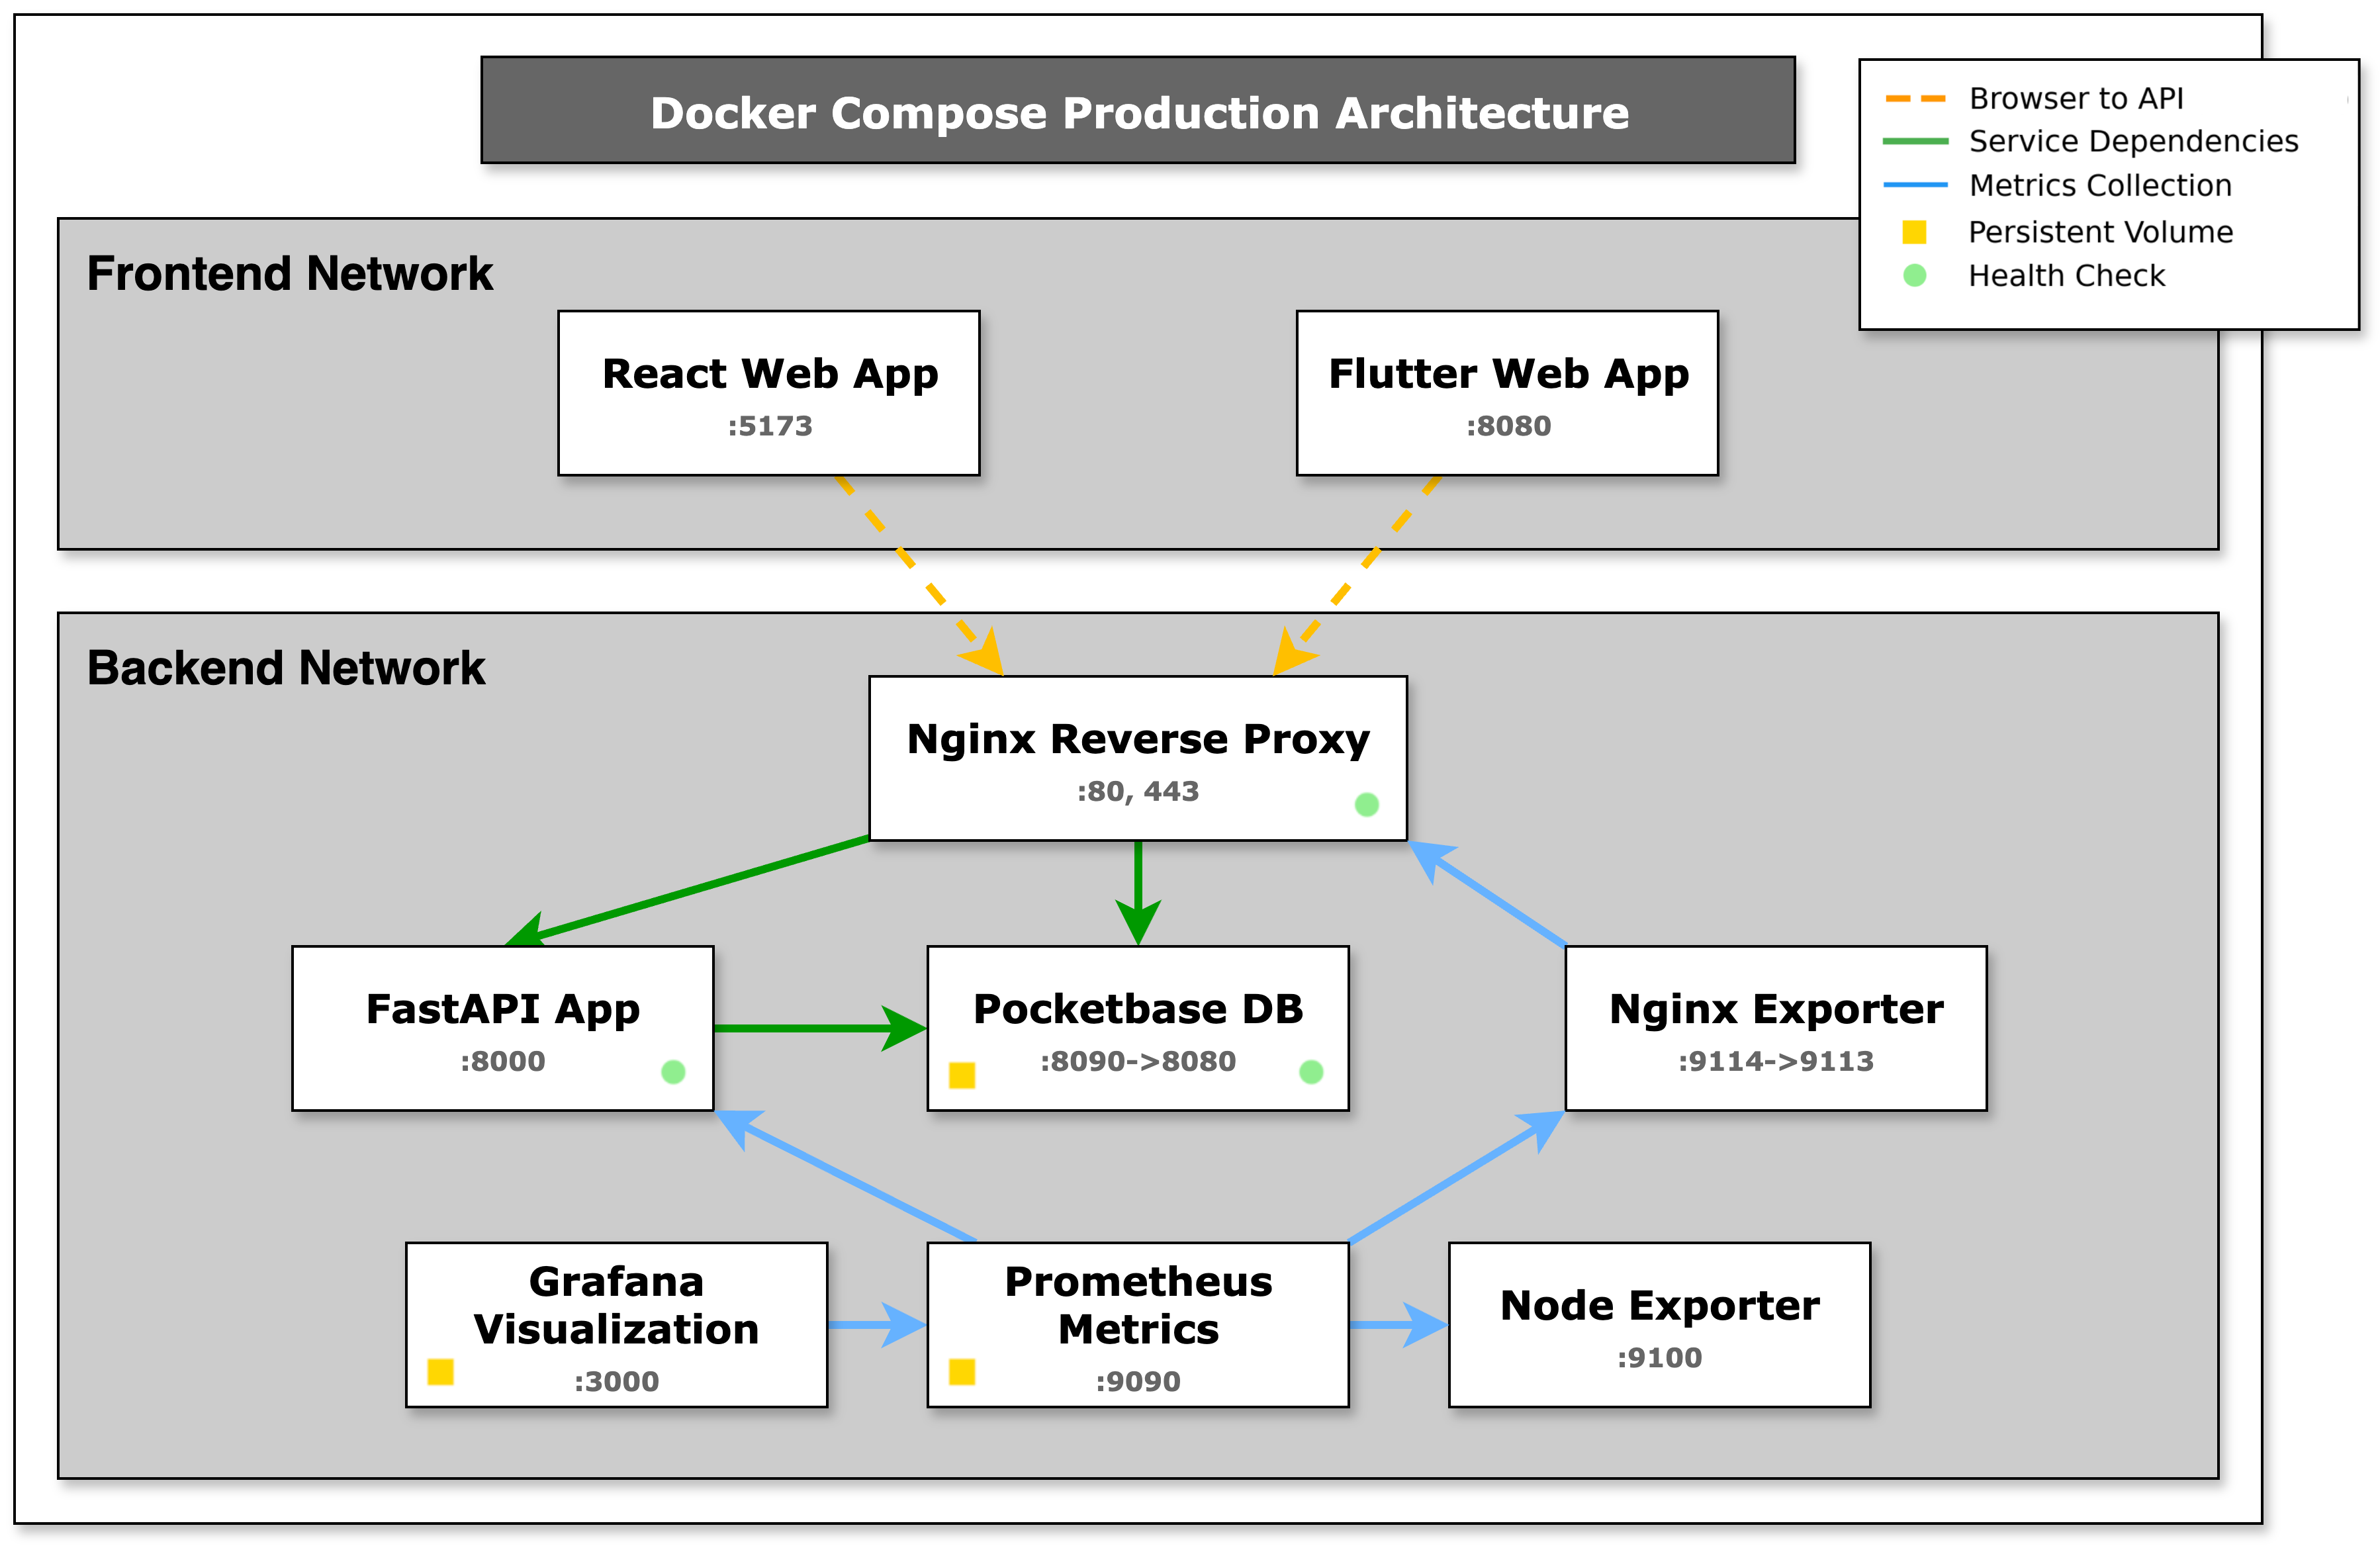
\includegraphics[width=\textwidth]{figs/chapter4/docker_architecture_diagram.png}
    \caption[Docker Compose Production Architecture]{Docker Compose Production Architecture: 9 Containerized Services with Nginx Reverse Proxy Routing}
    \label{fig:docker_architecture}
\end{figure}

The architecture separates concerns through service isolation while maintaining necessary communication pathways. Backend services operate within a dedicated network environment that provides service communication isolation and prevents external access to internal components. Frontend environments run independently, reflecting the distinct deployment lifecycles of client and server components. This separation enables independent scaling and updates without compromising system stability.

Service coordination relies on Docker Compose dependency management where FastAPI depends on PocketBase availability, and Nginx waits for both application services before accepting traffic. Health checks monitor each service at regular intervals, with automatic restart policies activating when failures occur to maintain availability.

Data persistence strategies balance durability requirements with operational flexibility through Docker volume management. PocketBase writes all data to the \texttt{pb\_data} volume, and Prometheus and Grafana maintain separate named volumes for metrics and dashboard configurations, isolating data from container lifecycles and ensuring information survives service updates and infrastructure changes.

\subsection{Operational Procedures} \label{subsection:operational_procedures}

Operational procedures were designed to balance deployment reliability with practical simplicity, Academic projects require reproducible deployment processes without complex operational expertise. The approach prioritizes automated validation through \texttt{docker-compose config} verification and systematic deployment using three-stage orchestration: configuration validation, image building, and detached service startup.

Configuration management separates sensitive credentials into \texttt{.env} files while frontend services receive environment variables directly from Docker Compose configurations. This separation enables secure credential distribution without requiring complex secret management infrastructure common in enterprise environments, while maintaining deployment simplicity for academic contexts.

Deployment orchestration follows a validation-first approach where \texttt{docker-compose config} prevents runtime failures through pre-deployment verification. Health checks must pass before routing traffic to newly deployed services, confirming service dependencies are resolved correctly and minimizing the risk of partial deployments that could compromise integrity.

Recovery procedures emphasize automated Docker restart policies over manual intervention: application services use \texttt{on-failure} restart policies while monitoring services run with \texttt{unless-stopped} to maintain availability. When network connectivity issues occur, the standard resolution involves \texttt{docker-compose down} followed by \texttt{docker-compose up} to recreate the Docker network, acknowledging that academic environments may lack continuous operational monitoring.

\section{Monitoring and Observability} \label{section:monitoring_observability}

Observability addresses the operational challenges of multi-service architectures, where system issues can emerge from complex component interactions. The monitoring strategy uses a layered approach that provides visibility while maintaining operational simplicity, prioritizing functional demonstration over operational complexity in the academic context.

The implementation prioritizes automated data collection through Prometheus scraping FastAPI metrics every 5 seconds and Node Exporter reading system statistics from host directories. Application monitoring captures request handling and processing times from the user perspective, while infrastructure monitoring provides insights into CPU, memory, and disk utilization across all containerized services.

Dashboard design provides technical visibility through four specialized Grafana dashboards: system overview tracking resource usage, application performance showing response times and error rates, AI performance monitoring, and infrastructure monitoring supporting capacity planning and troubleshooting. These dashboards enable administrators to assess operational status through visual metrics rather than manual inspection. Figure \ref{fig:docker_architecture} presents an example Grafana dashboard regarding PocketBase performance monitoring, during a simulated load test.

\begin{figure}[htbp]
    \centering
    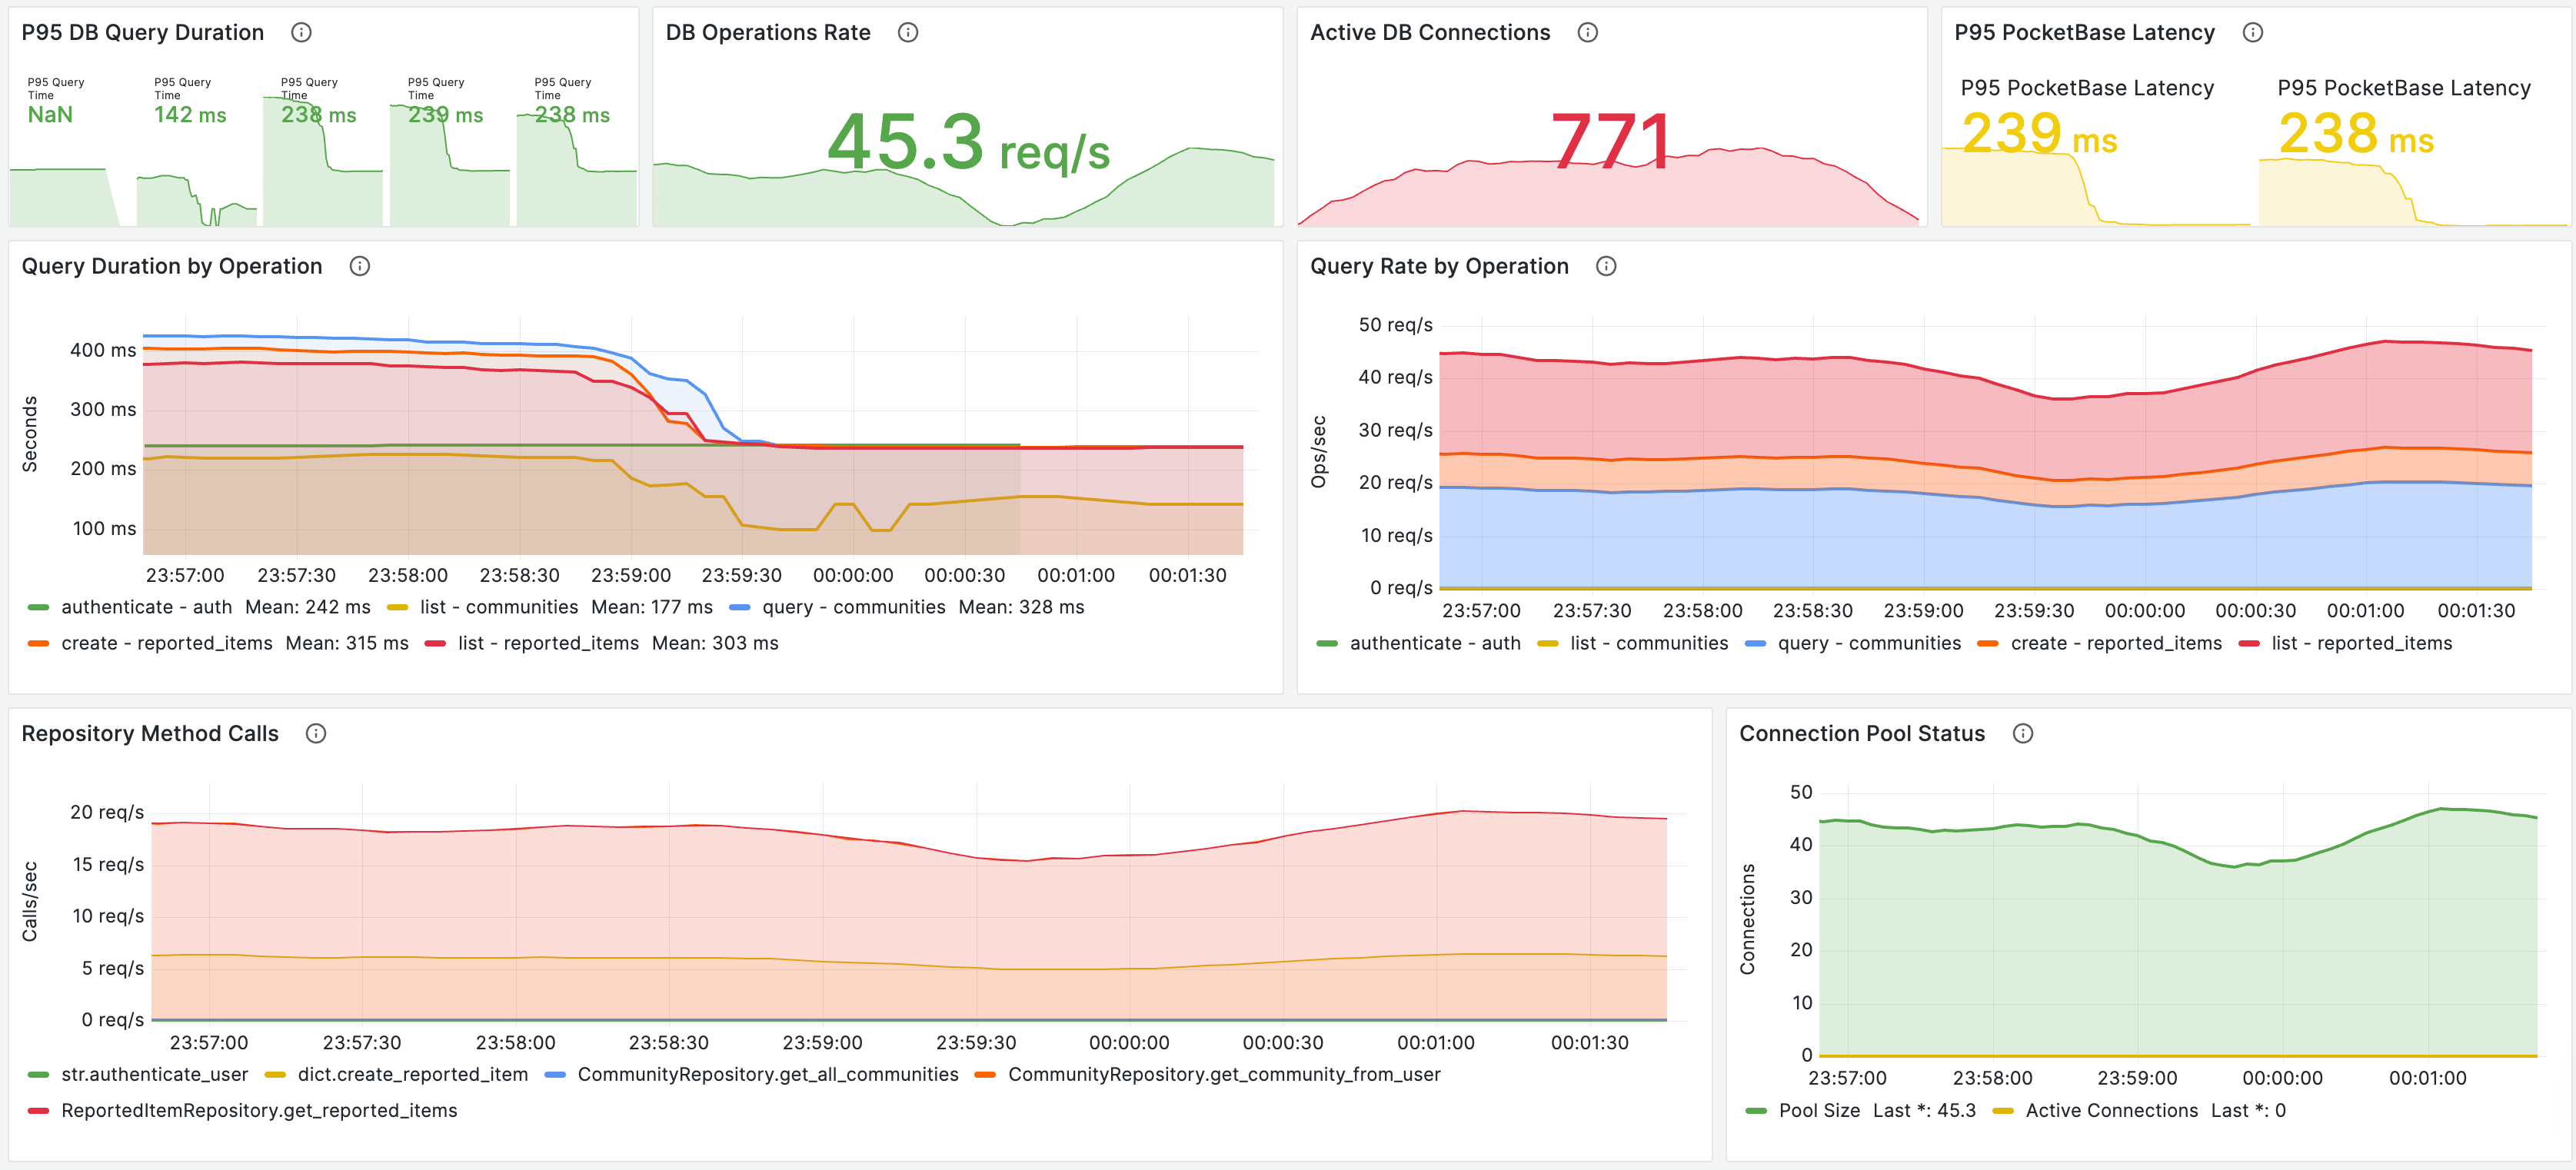
\includegraphics[width=\textwidth]{figs/chapter4/grafana_dashboard.png}
    \caption[Grafana Dashboard Monitoring]{Grafana dashboard monitoring PocketBase performance}
    \label{fig:docker_architecture}
\end{figure}

Data retention policies manage the balance between historical analysis capabilities and storage constraints through a 30-day Prometheus retention window. This automated lifecycle management prevents storage exhaustion while preserving 30 days of metrics history for trend analysis and capacity planning decisions in resource-conscious academic environments.

\section{Summary} \label{section:implementation_summary}

This chapter presented the implementation of the UAchado intelligent \ac{lfms}, showing how architectural decisions from Chapter \ref{chapter:methodology}  translated into a functional system. The implementation process validated key architectural choices and revealed practical considerations that influenced the final system design.

Database architecture focused on simplicity and development velocity by adopting a self-hosted backend platform rather than traditional database management. This approach worked well for rapid prototyping and community-based data isolation requirements. Multi-tenant design resolved scalability concerns and maintained clear organizational boundaries through community-based scoping.
    
Balancing performance requirements with operational complexity, service architecture decisions led to transitioning from planned microservices to a modular monolithic approach. This shift reflected practical constraints around deployment complexity and inter-service communication overhead. Authentication and security implementations followed industry standards for access control and minimized custom security code that could introduce vulnerabilities.

The \ac{ai} integration supports locally-hosted processing to address infrastructure reliability concerns common in academic environments. Multi-factor matching algorithm design balanced accuracy with computational efficiency, allowing the system to provide meaningful similarity scoring without requiring extensive computational resources.

Two distinct interfaces address different user interaction patterns through specialized implementations. The dual-platform approach recognized that administrative tasks benefit from desktop interfaces and field operations require mobile-first design. Technology selection focused on developer productivity and long-term maintainability over cutting-edge features.

Deployment architecture emphasized operational simplicity through containerization and integrated monitoring. These choices reduced infrastructure complexity and provided essential observability for production operations. The implementation demonstrates that thoughtful technology selection can deliver advanced functionality with reasonable operational overhead.